%%%%%%%%%%%%%%%%%%%%%%%%%%%%% TCC %%%%%%%%%%%%%%%%%%%%%%%%%%%%%%%%
%
% Template para TCC da Universidade Federal da Paraíba
%
% Autores: Elaine Soares elaineanita1@gmail.com
%          Rafael Brayner rafabrayner92@gmail.com
%          Roberto Júnior contato@robertojunior.net
%
% ShareLaTeX porting: Gustavo Sobral ghsobral@gmail.com
% 
% Revisão: Eudisley Anjos eudisley@ci.ufpb.br
%
% Sinta-se livre para melhorar e contribuir com esse projeto. 
%
%%%%%%%%%%%%%%%%%%%%%%%%%%%%%%%%%%%%%%%%%%%%%%%%%%%%%%%%%%%%%%%%%%%

\documentclass{tcc}

\begin{document}
\pagestyle{empty} %retira numeração da página
%Dados do TCC%
\author{Gabriel Machado Bandeira}
\title{Uma aplicação de Data Warehouse e mineração com base de dados de filmes}
\newcommand{\nomedocurso}{BACHARELADO EM CIÊNCIA DA COMPUTAÇÃO}
\newcommand{\orientador}{Prof. Dr. Jarley Palmeira Nóbrega}
\newcommand{\profa}{}
\newcommand{\profb}{}
\newcommand{\profc}{}
\newcommand{\insta}{\faculdade}
\newcommand{\instb}{\faculdade}
\newcommand{\instc}{\faculdade}
\newcommand{\coordenador}{Eduardo Calabria}
\newcommand{\departamento}{Nome do Departamento}

\begin{figure}[H]
\centering

\includegraphics[scale=2]{imagens/logo.png}
\end{figure}
\begin{center}
\textbf{\large{Faculdade Nova Roma}}\\
\textbf{\large{BACHARELADO EM CIÊNCIA DA COMPUTAÇÃO}}
\end{center}

\vspace{5em}

\begin{center}
\Large{\bf \MakeUppercase {\theauthor}}
\end{center}
\vspace{2em}
\begin{center}
\LARGE{\bf \MakeUppercase{\thetitle}}
\end{center}

\vfill






\vspace{2in}

\begin{center}
Recife, \MONTH, \the\year
\end{center}

\newpage
\begin{center}
\Large{\bf \MakeUppercase{\theauthor}}
\end{center}
\vspace{3in}
\begin{center}
\LARGE{\bf \thetitle}


\end{center}

\vspace{2in}

\begin{flushright}
Trabalho de Conclusão de Curso apresentado à \\Faculdade Nova Roma como pré-requisito parcial\\ para obtenção do título de Bacharel.\\
\vspace{0.2in}
Orientador: \orientador
\end{flushright}

\vfill
\begin{center}
\MONTH de \the\year
\end{center}

\newpage
\begin{center}
\Large{\bf \MakeUppercase{\theauthor}}
\end{center}
\vspace{3in}
\begin{center}
\LARGE{\bf \thetitle}
\end{center}

\vspace{0.05in}

\begin{flushright}
Trabalho de Conclusão de Curso apresentado à\\ Faculdade Nova Roma como pré-requisito parcial\\ para obtenção do título de Bacharel, sob orientação\\ do \orientador
\end{flushright}

\vspace{0.7in}

\hrule
\noindent Prof. Dr. \profa\\
\insta\\

\vspace{0.25in}

\hrule
\noindent Prof. Dr. \profb\\
\instb\\

\vspace{0.25in}

\hrule
\noindent Prof. Dr. \profc\\
\instc\\


\newpage

%Agradecimentos%
\section*{\centering{AGRADECIMENTOS}} 
Gostaria de agradecer primeiramente a minha mãe, Maria Alessandra Vieira Machado, tia, Adriana Vieira Machado e irmã, Giovanna Paula Machado Bandeira, que sempre me apoiaram nos momentos mais difíceis e nunca saíram do meu lado.

As minhas amigas, Ana Maria Raymundi, Gabriela Lopes Vasconcellos de Andrade e Marina Schoepping Falcão Cavalcante Lins, que me deram muita força e ajuda para completar este trabalho.

A todos meus amigos e amigas que, direta ou indiretamente, contribuíram para a conclusão desse trabalho.

Ao meu orientador, Jarley Palmeira Nobrega, a todo apoio e incentivo que me ajudaram muito.

A Faculdade Nova Roma, pela oportunidade de fazer o curso.



\newpage

%Resumo%
\section*{\centering{RESUMO}}
O trabalho realizado neste documento foi de análise de dados, tratamento de dados e de tentar prever a nota de um filme com base em dados colhidos de outros filmes. O intuito desse trabalho é de que qualquer pessoa com interesse em mineração de dados possa usar os resultados aqui colhidos para poder expandir as conclusões que foram tiradas. Nesse trabalho foi possível concluir que prever a nota de um filme requer bastante análise dos dados. Foi possível prever a nota com um erro relativamente pequeno.

{\bf Palavras-chave:} $<$Mineração de Dados$>$,  $<$Aprendizado de Máquina$>$, $<$Pentaho$>$, $<$WEKA$>$.
\section*{\centering{ABSTRACT}} 
The work made in this document was data analysis, data treatment and try to predict the score of a movie based on the data gathered from other movies. The main goal of this work is that any other person that has an interest in data mining can use the data results genereted here to expand the conclusions made. In this work was possible to conclude that predict the score of a movie requires a lot of data analysis. It was possible to predict the score with a small error.

{\bf Key-words:} $<$Data Mining$>$, $<$Machine Learnning$>$, $<$Pentaho$>$, $<$WEKA$>$.
\newpage

%Lista de figuras%
\renewcommand{\listfigurename}{\centering LISTA DE FIGURAS}
\listoffigures
\newpage

%Lista de tabelas%
\renewcommand{\listtablename}{\centering LISTA DE TABELAS}
\listoftables
\newpage

%Lista de abreviaturas%
\section*{\centering{LISTA DE ABREVIATURAS}} 

DW	–  	Data Warehouse

PDI	– 	Pentaho Data Integration 

WEKA	–	Waikato Environment for Knowledge Analysis

MSE    –   Mean Squared Error

RMSE    –   Root Mean Squared Error



\newpage

%Sumário%

\pagestyle{plain} %mostra numeração da página%
\tableofcontents

\newpage
\section{INTRODUÇÃO}

Existem diversas fontes de dados que podem conter algum tipo de conhecimento que não está visível aos nossos olhos, um certo padrão que não é tão fácil reconhecer sem alguma computação. A mineração de dados pode reconhecê-los e nos ajudar a decidir o que fazer com eles, como deixar um produto mais próximo de outro em um supermercado, pois um algoritmo de mineração descobriu que esses dois produtos são geralmente comprados em conjunto.

A mineração de dados pode estar ligada à inteligência artificial, já que métodos de aprendizado de máquina podem ser utilizados para encontrar padrões e nos auxiliar a descrever melhor o que foi encontrado.
Pensando nisso, o objetivo deste trabalho é utilizar a mineração de dados em uma base do IMDB (\textit{Internet Movie Database}) para tentar encontrar padrões que possam nos ajudar a prever a nota de filmes do IMDB.

Vários fatores podem levar ao fracasso ou ao sucesso de um filme, como não escolher bem os diretores, os atores, pouco investimento etc. O IMDB contém informações de filmes, séries e animações, e para cada um desses existe uma nota relacionada. Essa nota é atribuída pelos usuários e é geralmente levada em consideração ao se escolher um filme, afinal, não é tão comum alguém querer assistir um filme que tem uma nota muito baixa.

A possibilidade de prever essa avaliação dos usuários seria uma ferramenta útil durante a produção de um novo filme, os estúdios não gostariam que os seus filmes tenham péssimas avaliações e já podem trabalhar em cima do que foi previsto e possivelmente melhorar a nota.

Para isso, a mineração de dados irá se basear em dados históricos dos filmes para buscar encontrar algo que possa ajudar a melhorar a nota de um filme. Esse algo pode ser uma diretora especifica, línguas em que o filme foi lançado etc.

Visto isso, algumas hipóteses foram levantadas e os modelos foram usados para validá-las (ou não).

Para prever a nota de um filme baseado em dados históricos, aqui será discutido sobre a criação de Data Warehouses, que utiliza o processo de ETL (\textit{Extract, Transform, Load}), que será aplicado nesse trabalho, para serem criados. CRISP-DM, metodologia usada na mineração de dados e com uma visão de Bussiness Intelligence e uma ferramenta para auxiliar o ETL, o \pdi, junto com a linguagem de programação \textit{Python}.

Aqui também terá uma pequena introdução ao WEKA (\textit{Waikato Environment for Knowledge Analysis}), uma poderosa ferramenta para mineração de dados, com diversas formas de aplicar algoritmos em cima dos dados construídos.

Nesse capítulo, a motivação e os objetivos do trabalho foram apresentados. No Capítulo 2, uma visão geral sobre Data Warehouse será mostrada. No Capítulo 3, as principais características da plataforma Pentaho Data Integration serão introduzidas. Um breve resumo sobre o mineração de dados e a ferramenta WEKA é mostrado no Capítulo 4. O Capítulo 5 apresenta a metodologia utilizada no estudo de caso e também exibe e discute os principais resultados obtidos. A conclusão desse trabalho é apresentada no Capítulo 6.

\section{ Data Warehouse}
\subsection{O que é um Data Warehouse}
Para \citeAuthorPageYear{jmj}, um \textit{Data Warehouse} é um repositório de informações coletadas de múltiplas fontes, armazenado sobre um esquema definido e, geralmente, situado em um único local, no intuito de garantir a consistência dos dados caso eles sejam acessados de locais diferentes. Eles suportam o processamento de informações ao prover uma plataforma sólida de dados históricos para análise \citep{jmj}.

\subsection{Características de um Data Warehouse}
Segundo \citeAuthorPageYear{inmon}, um DW é um conjunto de dados orientado por assuntos, integrado, variável com o tempo e não volátil, criados para dar suporte à decisão.

Orientado por assunto, ou seja, organizado em torno de um assunto principal. Em vez de se concentrar nas operações diárias e no processamento de transações de uma empresa, um DW foca na modelagem e análise de dados para tomadores de decisões \citep{jmj}.
Integrado, um DW contém informações de fontes heterogêneas, como base de dados relacionais e \textit{flat files}. Processos de \textit{data integration} e \textit{data cleaning} são aplicados para garantir a consistência dos dados \citep{jmj}.

Variável com o tempo, armazena informações históricas dos últimos 5-10 anos, por exemplo. Toda estrutura chave em um DW contém um elemento de tempo \citep{jmj}.
E por último, não volátil, os dados não precisam ser alterados, já que um DW é fisicamente separado do ambiente operacional. As únicas operações executadas em um DW são: carga inicial e acesso aos dados \citep{jmj}.

\subsection{Modelos de Data Warehouse}
Para \citeAuthorPageYear{jmj}, um DW pode ser dividido em três modelos: \textit{enterprise warehouse}, \textit{data mart} e \textit{virtual warehouse}.

\subsubsection{Enterprise Warehouse}
\citeAuthorPageYear{jmj} diz que um \textit{enterprise warehouse} coleta informações sobre um assunto que abrange toda uma organização. Ele fornece integração de dados em escala corporativa, geralmente de um ou mais sistemas operacionais ou de provedores de informação externos. Ele contém dados detalhados e sumarizados e podem variar de alguns poucos \textit{gigabytes} para centenas de \textit{gigabytes}.

Um \textit{enterprise warehouse} é um conglomerado das \textit{data warehouse staging} e \textit{presentation areas} de uma organização \citep{kimball2002}


\subsubsection{Data Mart}
Conforme \citeAuthorPageYear{jmj} diz, um \textit{data mart} contém um subconjunto de dados de uma escala corporativa e tem o escopo limitado a assuntos específicos.

Os \textit{data marts} são frequentemente implementados em servidores de baixo custo e têm o seu ciclo de implementação medido em semanas, em vez de meses ou anos. Os dados podem ser independentes ou dependentes. Caso sejam independentes, vão ter como fonte um ou mais sistemas operacionais ou provedores de informação externos. No caso de serem dependentes, os dados contidos no \textit{data mart} serão fornecidos diretamente de um \textit{enterprise warehouse}.

\subsubsection{Virtual Warehouse}
\citeAuthorPageYear{jmj} dizem que as \textit{virtual warehouses} são um conjunto de \textit{views} em cima dos bancos de dados operacionais. Eles podem manter um processamento eficiente de \textit{queries} exibindo apenas alguns dos possíveis sumários. Ele também é de fácil construção.

\subsection{Componentes}

A figura \ref{dwComponents} mostra quais são os componentes de um DW, explicados com detalhes mais abaixo.
\begin{figure}[H]
\centering
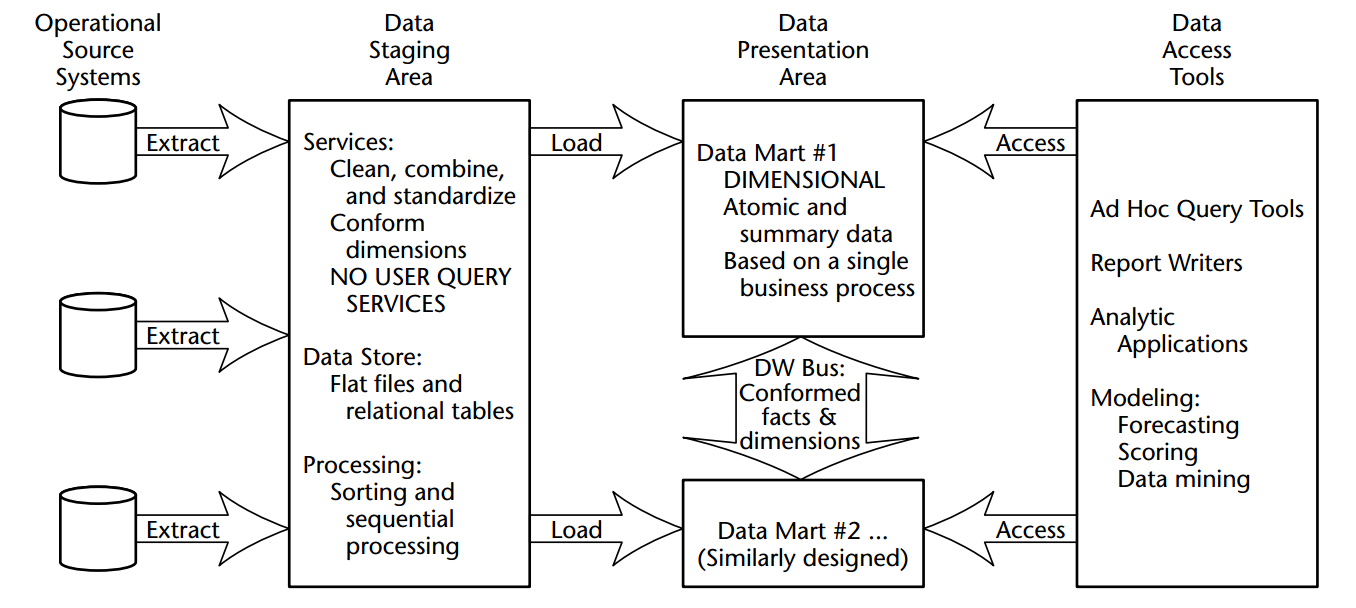
\includegraphics[height=5cm]{imagens/componentes_DW.png}
\caption{Componentes de um Data Warehouse (\citeauthor{kimball2002} \citeyear{kimball2002})}
\label{dwComponents}
\end{figure}

\subsubsection{Operational Source Systems}
Fontes de Dados Operacionais, nas palavras de \citeAuthorPageYear{kimball2013}, são responsáveis pela captura de transações de negócio. Esses sistemas são mantidos fora do \textit{data warehouse} porque se tem pouco ou nenhum controle sobre o conteúdo ou formato dos dados. Eles processam performance e disponibilidade. \citeAuthorPageYear{kimball2013} também afirmam que esses sistemas mantêm poucos dados históricos. Um bom \textit{data warehouse} pode reduzir a necessidade dos sistemas de dados operacionais de representarem o passado. Em muitos casos, eles são de algum propósito especial, sem responsabilidade de compartilhar dados comuns, como dados de produtos, clientes etc \citep{kimball2013}.

\subsubsection{Data Staging Area}
\citeAuthorPageYear{kimball2002} sugerem que a \textit{staging area} é tanto uma área de armazenamento como um conjunto de processos conhecidos como \textit{extract-transformation-loading} (ETL). Esse processo será melhor explicado mais pra frente. Eles ainda falam que a \textit{staging area} é tudo entre os \textit{operational source systems} e a \textit{presentation area}. 

Existem diversas formas de carregar dados na \textit{staging area}, como \textit{flat files}, xml, modelos relacionais. Ela regularmente é composta de um \textit{database management system} (DBMS) e arquivos de texto (\textit{flat files}) \citep{kimball2004}. Em muitos casos, os dados precisam ser armazenados fora de um DBMS, em \textit{flat files}, para um rápido processamento sequencial \citep{kimball2004}.
\citeAuthorPageYear{kimball2002} descrevem o primeiro passo na criação (extração) de um \textit{data staging area} como a leitura e entendimento da fonte de dados e copiar o que for necessário para manipulação futura. \citeAuthorPageYear{kimball2002} afirma que quando os dados são extraídos, existem diversas transformações que podem ser feitas, como limpeza, combinação de dados de diferentes fontes, remoção dados duplicados etc. Essas transformações acontecem antes de se carregar os dados na \textit{presentation area}.

\subsubsection{Data Presentation Area}
A \textit{presentation area}, ou área de apresentação, é onde os dados estão organizados, armazenados e disponíveis para consulta por usuários ou alguma aplicação analítica de \textit{Business Intelligence} (BI) \citep{kimball2013}. Tudo que o negócio vê e toca é através das ferramentas de acesso ou aplicações de BI.

Os dados devem ser, de acordo com \citeAuthorPageYear{kimball2013}, apresentados, armazenados e acessados através de esquemas dimensionais, sejam eles esquemas estrela ou cubos OLAP. Eles devem conter dados atômicos detalhados \citep{kimball2013}.  Embora a \textit{presentation area} contenha dados agregados, é completamente inaceitável que somente dados sumarizados sejam armazenados enquanto os dados atômicos estão trancados em modelos normalizados. \citep{kimball2013}. Os dados mais finamente granulados devem ser apresentados na \textit{presentation area} para que usuários possam fazer as perguntas mais precisas.

A área de apresentação deve ser estruturada ao redor dos processos de medição de eventos, isso se alinha naturalmente com os \textit{operational source data capture systems}. Os modelos dimensionais devem corresponder aos eventos de captura de dados, não devem entregar um "relatório do dia" \citep{jmj}. 

\subsubsection{Data Access Tools} Ferramentas de Acesso de Dados, ou \textit{Data Access Tools}, são ferramentas usadas para consultar área de apresentação. Uma ferramenta dessas pode ser tão simples quanto \textit{Queries Ad Hoc} ou tão complexa quanto uma ferramenta de mineração de dados ou modelagem \citep{kimball2013}. 

\subsection{Extract, Transform, Load (ETL)}
O processo de \textit{extract, transform, load} (extrair, transformar, carregar), mais conhecido como ETL, é um processo utilizado para a construção de um DW, contendo os passos que são mostrados na figura \ref{etl}. 
\begin{figure}[H]
\centering
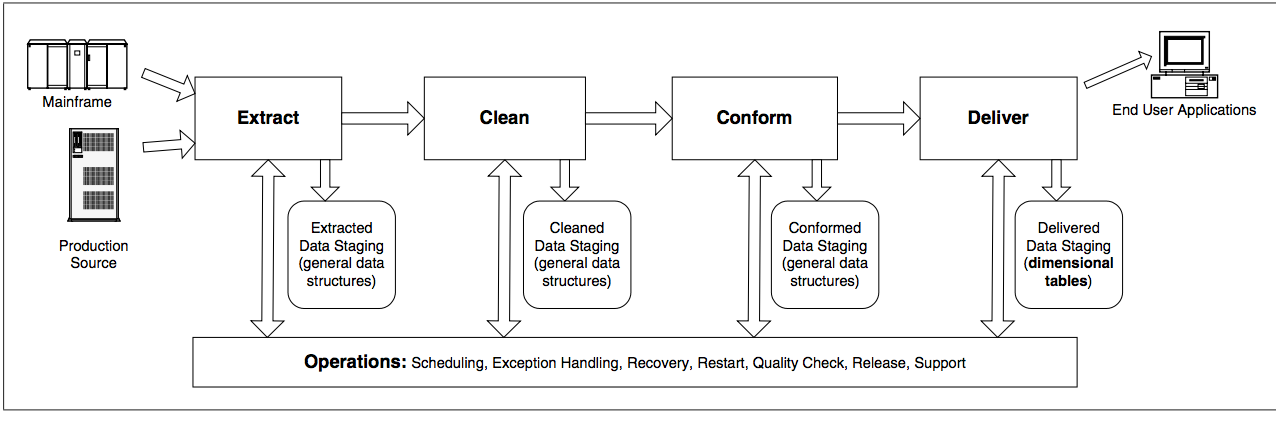
\includegraphics[height=5cm]{imagens/dw_process.png}
\caption{Processo de ETL (\citeauthor{kimball2004} \citeyear{kimball2004})}
\label{etl}
\end{figure}
O primeiro passo é a extração dos dados: espera-se que o sistema tenha que extrair dados de uma grande variedade de fontes \citep{kimball2013}. As organizações podem extrair dados de fontes como arquivos xml, banco de dados, planilhas etc.

O segundo passo é a transformação: após os dados serem extraídos, diversas transformações podem ser executadas, como limpeza, que irá remover alguns ruídos, combinação de dados de fontes diversas (bancos de dados, \textit{data warehouses}, arquivos csv, planilhas, etc) e tratar dados duplicados\citep{kimball2013}. Essa limpeza pode, nas palavras de \citeAuthorPageYear{kimball2013}, mudar os dados e aperfeiçoar o seu valor para uma organização.

O terceiro e último passo é o carregamento, que é o processo de estruturar fisicamente e carregar os dados dentro dos modelos dimensionais da \textit{presentation area} \citep{kimball2013}.

\subsection{Modelagem Dimensional}
A modelagem dimensional permite que os usuários do negócio enxerguem os dados com facilidade, ao entregar dados entendíveis e uma performance rápida, com dados visualizados em dimensões.

Existem quatro etapas para a construção de um modelo dimensional, sendo elas: \textbf{selecionar o processo de negócio}, \textbf{declarar o grão}, \textbf{identificar as dimensões} e \textbf{identificar os fatos}. 

Segundo \citeAuthorPageYear{kimball2013}, os processos de negócio são as atividades operacionais realizadas por uma organização. É um processo importante, pois define como o grão, dimensões e fatos serão declarados. O grão estabelece o que uma única linha na tabela de fatos representa \citep{kimball2013}.

\subsubsection{Tabela de Dimensões}
De acordo com \citeAuthorPageYear{kimball2013}, as dimensões fornecem o contexto de "quem, o que, onde, quando e como" de cada processo do negócio. As tabelas de dimensões podem incluir diversas colunas, mas costumam ter menos dados que a tabela de fatos. Elas têm chave primária, que vai permitir o relacionamento com a tabela de fatos.
\citeAuthorPageYear{kimball2013} afirmam que a tabela de dimensões pode ser conhecida como a "alma" de um sistema de DW, pois contém dados que permitem que o sistema de DW seja alavancado.

\subsubsection{Tabela de Fatos}
A tabela de fatos armazena as métricas resultantes de um processo de negócio de uma organização \citeAuthorPageYear{kimball2013}. Cada linha em uma tabela de fatos representa um evento de medição. Os dados, em um nível especifico de detalhe, podem ser chamados de grãos, como apenas uma linha por produto vendido \citep{kimball2013}.

Os dados mais úteis são os numéricos e aditivos. Aditividade é importante, pois dificilmente irá se fazer uma consulta que traga apenas uma linha, mas sim trará centenas, milhares ou milhões de dados e a coisa mais útil para se fazer com eles é somar \citep{kimball2013}.

\citeAuthorPageYear{kimball2013} falam que é possível manter dados textuais em uma tabela de fatos, eles são comumente usados para descrever algo e estão em uma lista discreta de valores. 

As tabelas de dimensões, conforme \citeAuthorPageYear{kimball2013}, têm uma ou mais chaves estrangeiras, que irá se ligar as chaves primarias das tabelas de dimensões. Eles afirmam que a tabela de fatos tem sua própria chave estrangeira, que é um subconjunto das chaves estrangeiras, chamado de chave composta. 

\subsubsection{Esquema Estrela}
Esse esquema, mostrado como exemplo na figura \ref{star}, armazena os dados em uma arquitetura semelhante a uma estrela, onde cada ponta é uma dimensão e todas se relacionam com a tabela de fatos, como mostra a figura. \citeAuthorPageYear{jmj} mostram que a tabela de fatos contém chaves para todas as outras tabelas assim como dados de medidas.
\begin{figure}[ht]
\centering
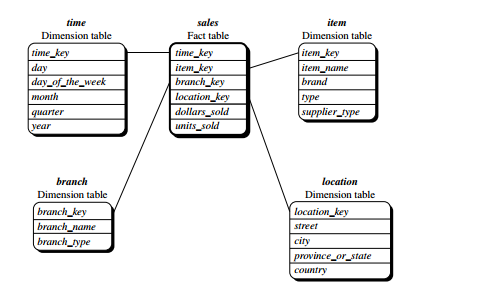
\includegraphics[height=6.2cm]{imagens/starscheme.png}
\caption{Esquema Estrela (\citeauthor{jmj} \citeyear{jmj})}
\label{star}
\end{figure}
\\
\subsubsection{Esquema Snowflake}
\begin{figure}[ht]
\centering
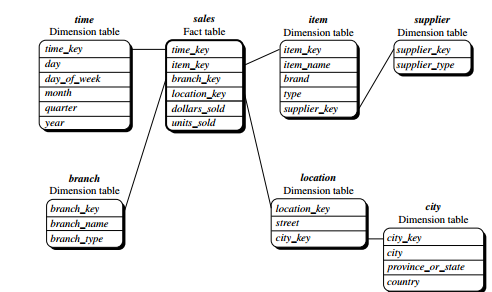
\includegraphics[height=6.2cm]{imagens/snowflakescheme.png}
\caption{Esquema Snowflake (\citeauthor{jmj} \citeyear{jmj})}
\label{snowflake}
\end{figure}
\subsubsection{Cubo e OLAP}
Conforme \citeAuthorPageYear{jmj}, DW e ferramentas OLAP são baseados no modelo multidimensional e ele visualiza os dados no formato de cubos de dados, como mostra a figura \ref{cube}. Um cubo permite visualizar os dados em diversas dimensões simultaneamente.
\begin{figure}[ht]
\centering
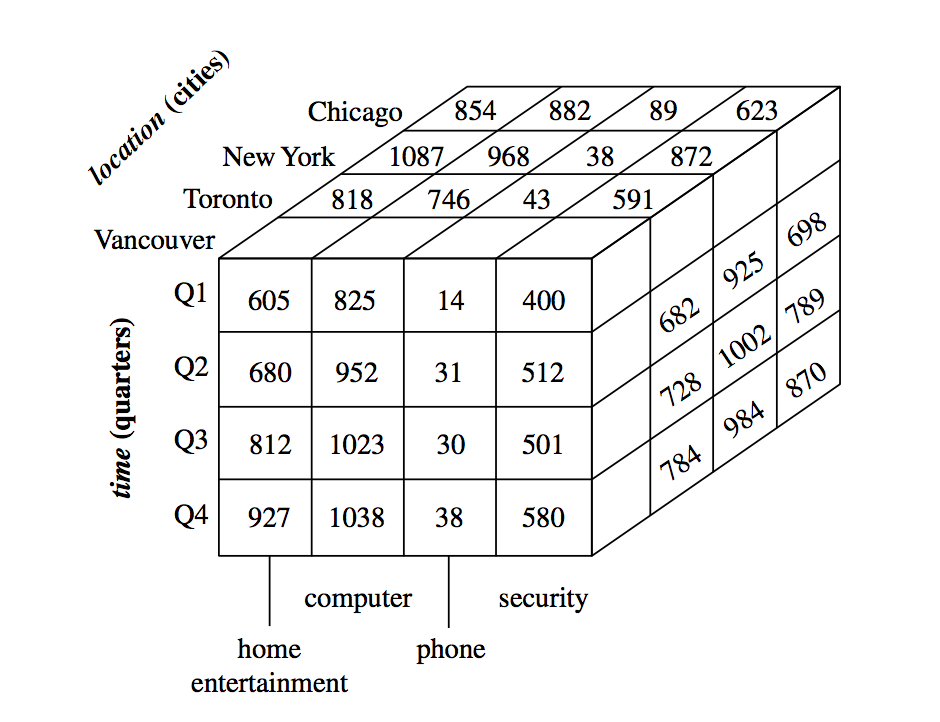
\includegraphics[height=6.2cm]{imagens/datacube.png}
\caption{Exemplo de um cubo de dados (\citeauthor{jmj} \citeyear{jmj})}
\label{cube}
\end{figure}
Dimensões são entidades que uma organização quer manter os dados \citep{jmj}. Uma dimensão deve ter uma tabela associada, a tabela de dimensões.


\citeAuthorPageYear{kimball2013} dizem que os modelos dimensionais implementados em base de dados multidimensionais são chamados de \textit{online analytical processing (OLAP) cubes}. Diversas operações estão associadas a esses cubos, como \textit{roll up, drill down, slice and dice e pivot}

\begin{itemize}
    \item \textbf{roll-up}: segundo \citeAuthorPageYear{jmj}, a operação de \textit{roll-up} executa agregações em um cubo de dados ou por \textit{subir em uma hierarquia conceitual} de uma dimensão ou por redução dimensional. Quando essa operação é realizada, uma ou mais dimensões podem ser retiradas do cubo.
    
    \item \textbf{drill-down}: Essa operação é a inversa da \textit{roll-up}, indo de dados menos detalhados para dados mais detalhados. Pode ser feito ou por \textit{descer uma hierarquia conceitual} de dimensões ou \textit{introduzir dimensões adicionais} \citep{jmj}
    
    \item \textbf{slice and dice}: A operação \textbf{slice} faz uma seleção em uma subdimensão do cubo, resultando em um subcubo \citep{jmj}. A operação \textbf{dice} cria um subcubo ao efetuar uma seleção em uma ou mais dimensões \citep{jmj}.
    
    \item \textbf{pivot}: \citeAuthorPageYear{jmj} dizem que \textit{pivot} (ou rotate) é uma operação que permite mover o cubo em algum eixo permitindo uma exibição dos dados em de uma forma alternativa.
\end{itemize}

\section{Pentaho Data Integration}
Nas seções anteriores foi discutido um pouco das principais características de um Data Warehouse e do processo CRISP-DM. Nessa seção, será discutida a utilização do Pentaho Data Integration (PDI) no processo de ETL, como ela pode ser aplicada e suas principais características.
O PDI, também conhecido como Kettle, oferece diversas ferramentas para a extração de dados de fontes diversas, transformações, limpezas e de carregamento dos dados
\subsubsection{Arquitetura}
O \pdi é composto basicamente de quatro componentes:
\begin{itemize}
    \item Spoon: é uma aplicação desktop de interface gráfica para a criação de jobs e transformations. Permite a criação de processos de ETL sem a necessidade de programação;
    \item Pan: uma interface de linha de comando que pode ser usado para a execução de jobs;
    \item Kitchen: interface de linha de comando que pode ser usada para a execução de jobs;
    \item Carte: uma aplicação web que permite a utilização de um servidor de ETL remoto, fornecendo capacidades de execução remota similares ao servidor de Data Integration.
\end{itemize}

\subsubsection{Princípios de Design}
\citeAuthorPageYear{kettle} dizem que o Pentaho foi desenvolvido com alguns princípios de design fundamentais, eles são. Algumas experiências negativas levaram a essas decisões.

Ele é de fácil desenvolvimento, não é necessário se preocupar com instalação de software. Segundo \citeAuthorPageYear{kettle}, várias ferramentas baseadas em Java precisavam que o usuário especificasse explicitamente qual era o nome da Classe Java de Driver e a URL do JDBC, apenas para criar uma conexão com o banco de dados. O Kettle sempre tentou ficar longe desses problemas \citep{kettle}. Ele evita a necessidade de programar, toda linha de código adiciona complexidade e custo de manutenção ao projeto, então faz sentido não ter que lidar com isso \citep{kettle}.

Ele mantém as funcionalidades disponíveis na interface de usuário, \citeAuthorPageYear{kettle} dizem que é possível realizar ETL por XML, repositório ou uma API. E todas essas opções também estão disponíveis em uma interface gráfica. Sem limitações de nomenclatura, as ferramentas de ETL precisam ser inteligentes para lidar com qualquer tipo de identificador, isso permite que a solução seja auto descritiva e reduzindo parcialmente a necessidade de documentação \citep{kettle}.

\citeAuthorPageYear{kettle} dizem que permitir que qualquer pessoa veja o que está acontecendo nas várias partes de um processo de ETL é crucial, permite acelerar o desenvolvimento e reduzir o custo. Fluxo de dados flexível, o \pdi foi criado para ser o mais flexível possível, respeitando os fluxos que podem ser criados \citep{kettle}. Apenas mapear dados impactados, \citeAuthorPageYear{kettle} dizem que um dos princípios fundamentais do Kettle é todos os campos que não são mapeados passam automaticamente para o próximo passo do processo, reduzindo assim o custo de manutenção.

\subsubsection{Processo}
Ao abrir o \pdi, ele apresenta a página inicial, como mostra na figura \ref{initialpdi}. Dessa tela é possível criar \textit{Jobs} e \textit{Transformations}, que serão explicados mais pra frente. 
\begin{figure}[H]
\centering
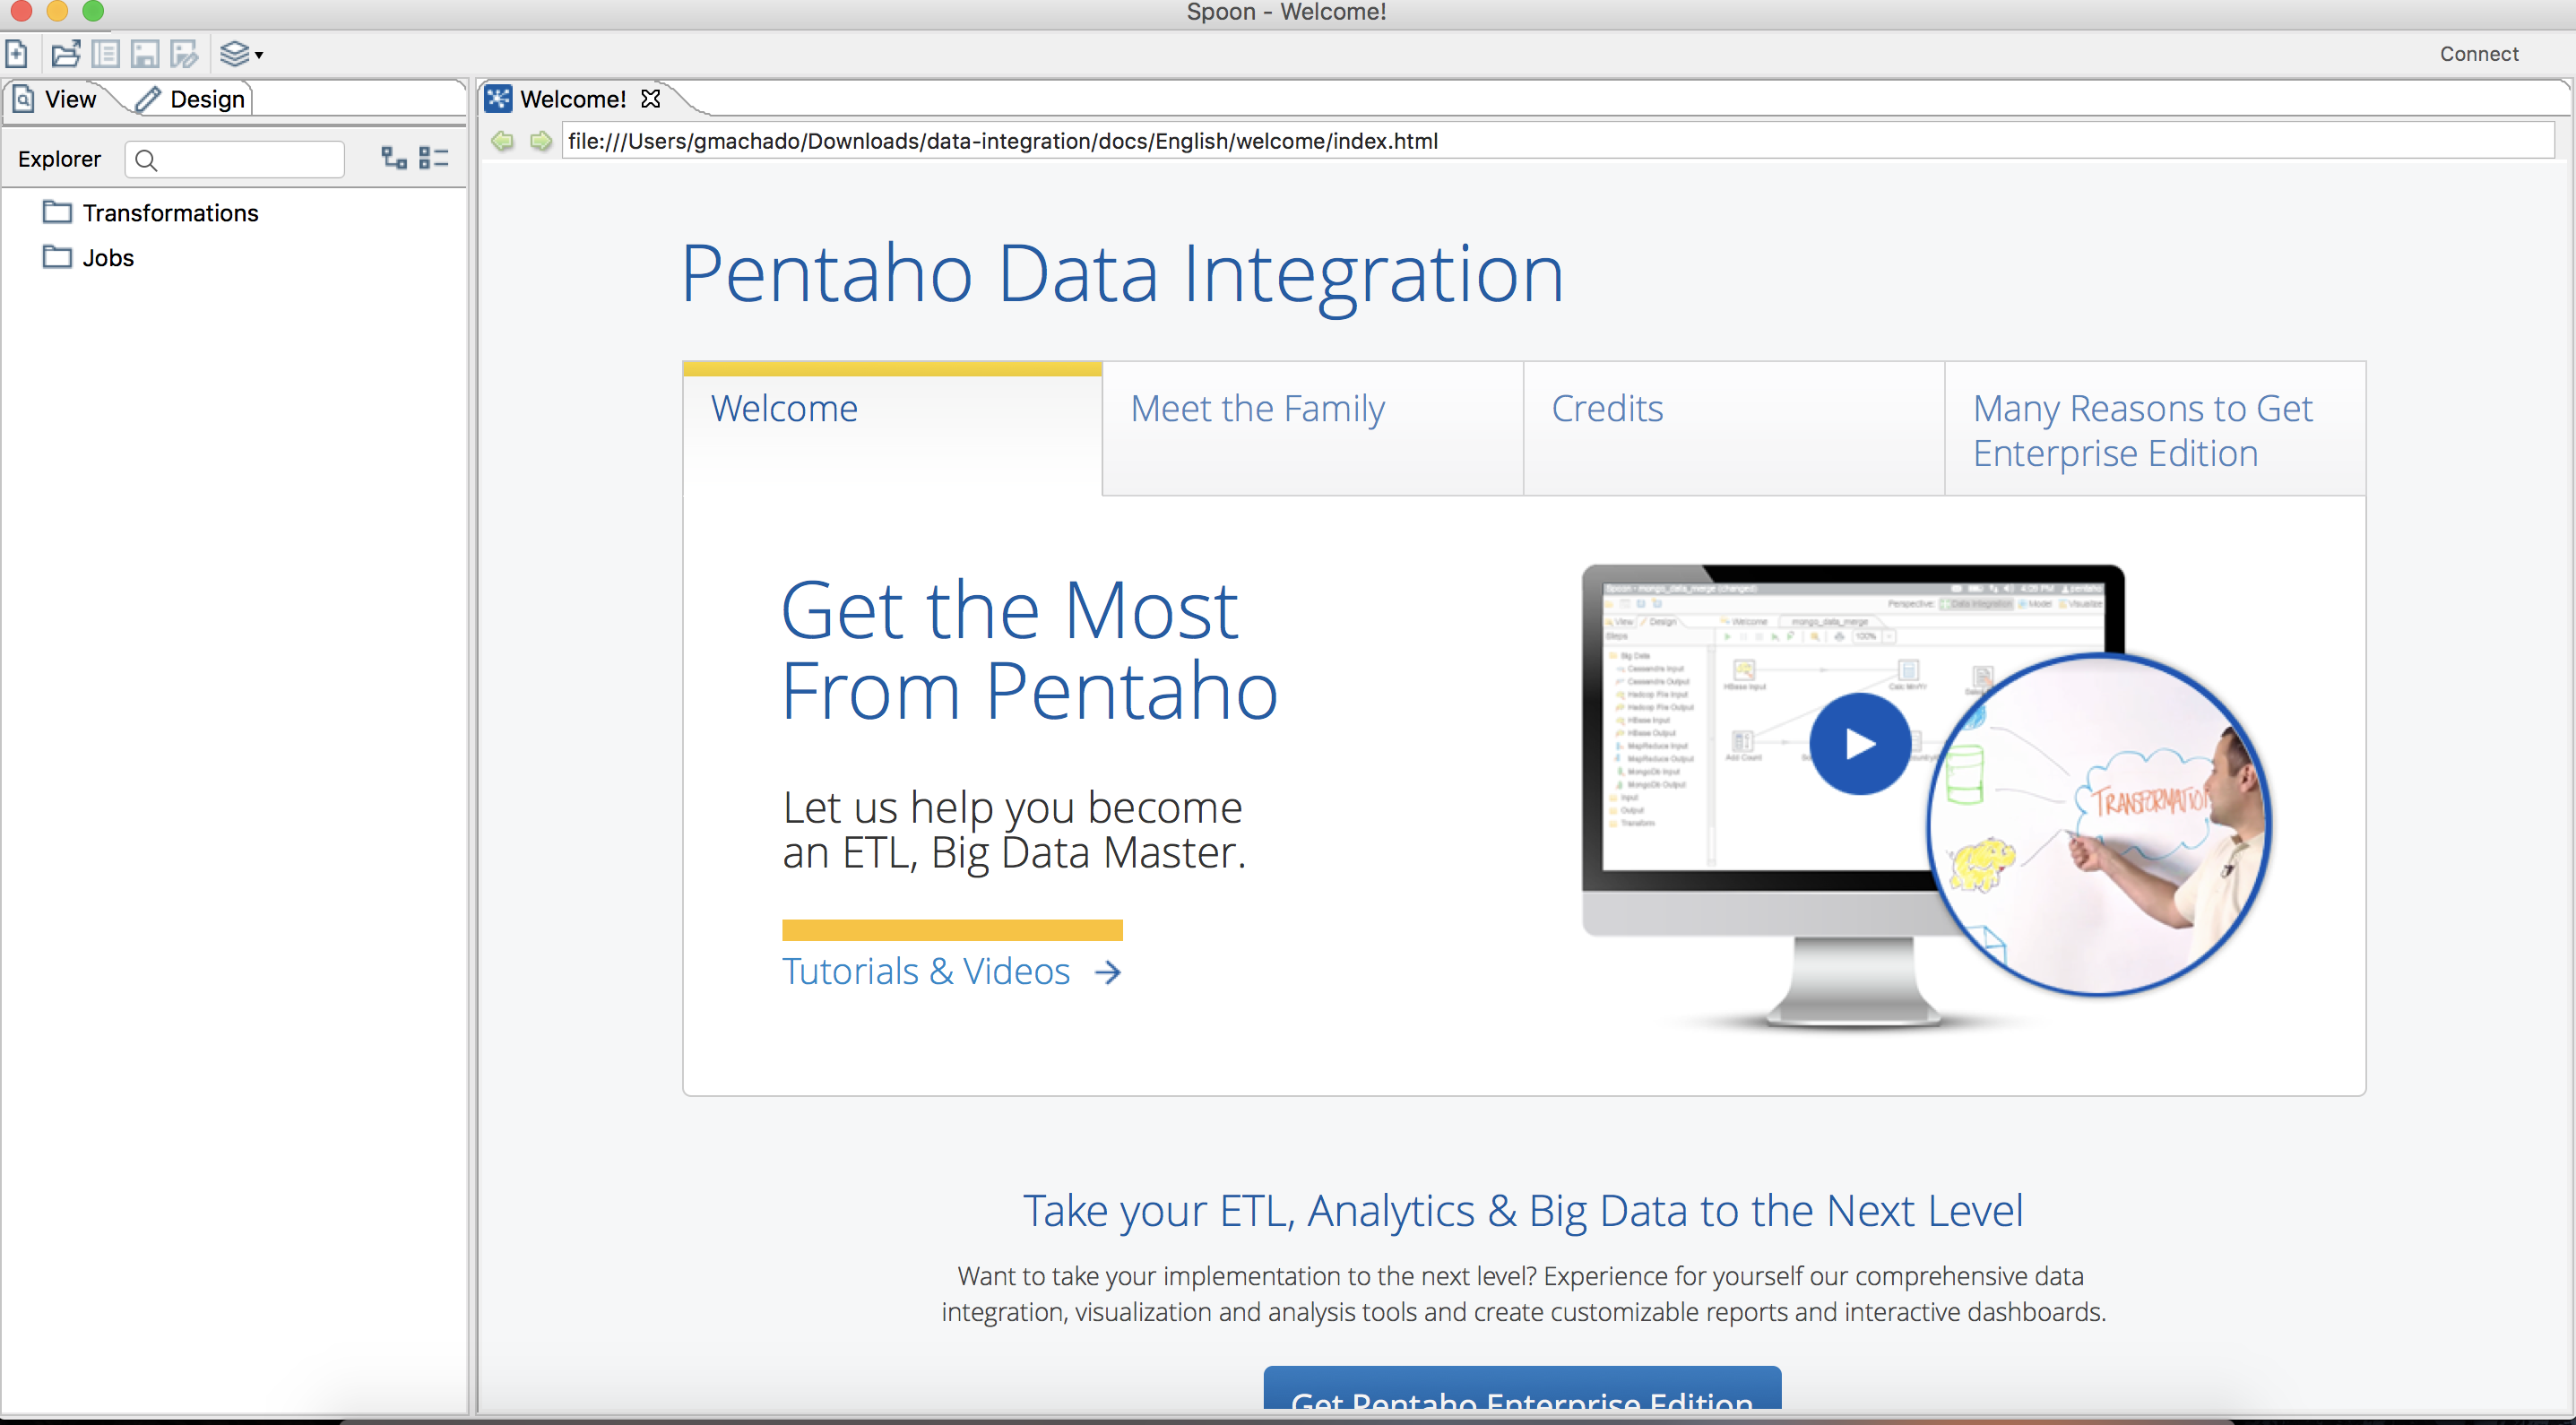
\includegraphics[height=5cm]{imagens/pagina_principal_pentaho.png}
\caption{Página inicial do \pdi}
\label{initialpdi}
\end{figure}
O \pdi utiliza \textit{transformations} que pode contém uma série de \textit{steps} e \textit{jobs} para realizar o processo de ETL. A figura \ref{transformationOptions} mostra algumas das opções para criação de transformations.
\begin{figure}[H]
\centering
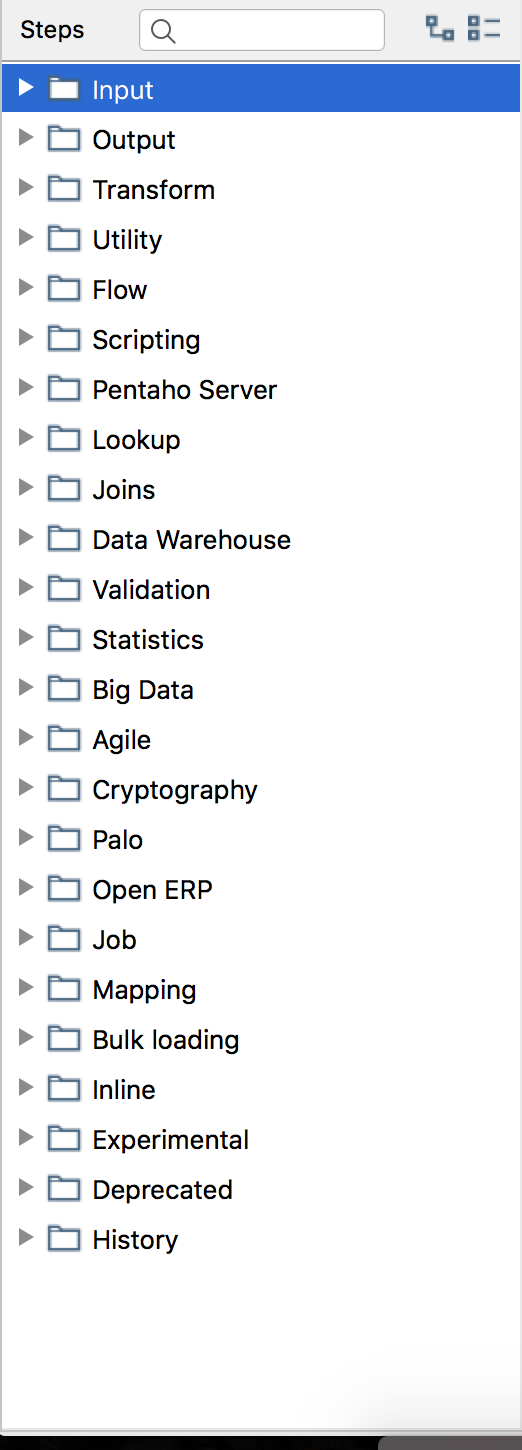
\includegraphics[width=4cm, height=8cm]{imagens/opcoes_de_transformacao.png}
\caption{Opções de transformações}
\label{transformationOptions}

\end{figure}
Transformation, segundo \citeAuthorPageYear{kettle}, consiste em um ou mais \textit{steps} que realiza a leitura de arquivos, filtrar linhas, limpeza dos dados e carregamento dos dados em uma base de dados. Os \textit{steps} são conectados por \textit{hops}, que são caminhos de um único sentido por onde os dados trafegam. 

\begin{figure}[H]
\centering
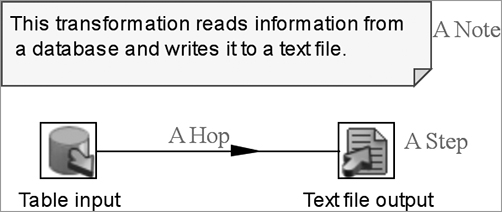
\includegraphics[height=5cm]{imagens/transformation.png}
\caption{Transformation (\citeauthor{kettle} \citeyear{kettle})}
\label{transformation}
\end{figure}

A figura \ref{transformation} mostra um pequeno exemplo pequeno de uma \textit{transformation} no \pdi.

Um \textit{step} é representado graficamente por um bloco, eles precisam ter um nome único. \citeAuthorPageYear{kettle} dizem que um step é capaz de ler e de escrever linhas de dados. Os steps escrevem dados nos \textit{outcoming hops}, que são conectados a um ou mais steps no final do hop, esse hop é chamado de \textit{incomming hop} os dados são lidos nos incoming hops. Além disso, um cada step tem uma capacidade diferente, como a figura acima mostra, que o o primeiro irá receber dados de uma tabela e o segundo irá escrever os dados em um arquivo.

Um \textit{hop} é representado por uma seta ligando dois steps, que define o fluxo dos dados entre eles \citep{kettle}. Um hop também representa um buffer de dados, chamado de row set, que quando está cheio, o step que escreve os dados para e quando está vazio, o step que lê os dados aguarda até que mais dadas sejam escritos.

Os jobs são um conjunto de um ou mais \textit{jobs entries} que são executados em uma certa ordem. A figura \ref{jobsOptions} mostra algumas opções que podem ser utilizadas para criar jobs. Os job entries, assim como os steps, são passos que são executados. Eles são conectados utilizando \textit{job hops}, que definem o caminho de execução entre os job entries \citep{kettle}.
\begin{figure}[H]
\centering
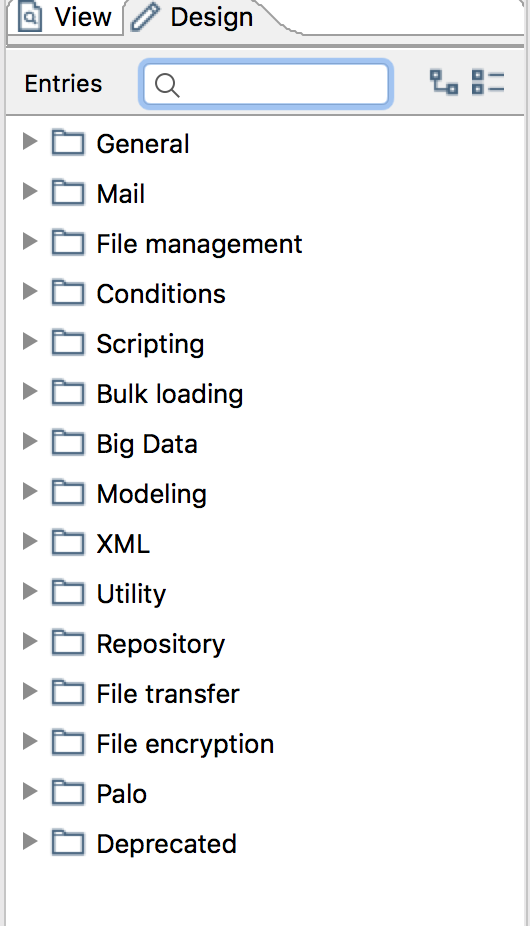
\includegraphics[width=7cm, height=9cm]{imagens/opcoes_de_jobs.png}
\caption{Opções de Jobs}
\label{jobsOptions}
\end{figure}
\subsubsection{Extract}
O \pdi oferece ferramentas para extração dos dados de fontes como arquivos de texto, planilhas, metadados, xml, banco de dados. Como mostrado na figura \ref{inputOptions}, a opção \textit{input} tem várias opções para realizar a entrada de dados. \\
\begin{figure}[H]
\centering
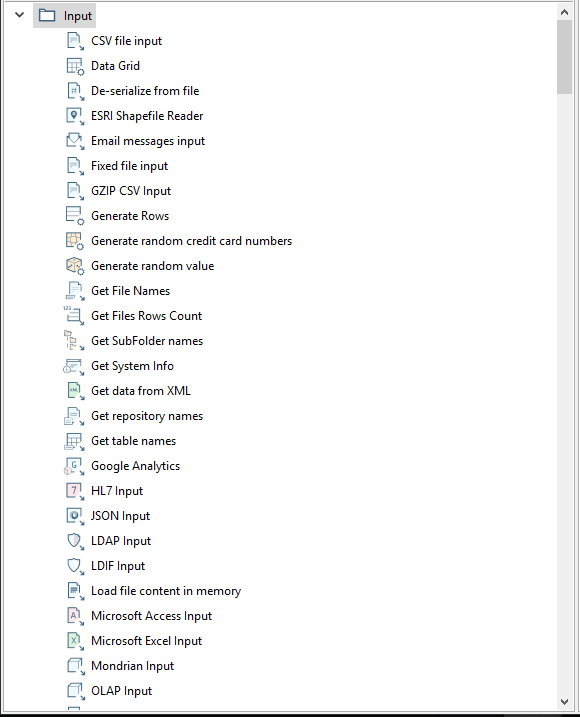
\includegraphics[width=7cm, height=9cm]{imagens/input.png}
\caption{Steps da categoria input}
\label{inputOptions}
\end{figure}
Um dos \textit{steps} responsáveis pela extração é o \textit{Text file input}, que recebe um arquivo de texto, geralmente csv, e consegue fazer a extração dos campos desejados.
No exemplo abaixo, um arquivo foi carregado com as informações da tabela \ref{autores}:\\
\begin{table}[H]
\centering
\caption{ Autores }
\vspace{0.2in}
\newcolumntype{C}{>{\centering\arraybackslash}X}%
\newcommand{\rowstyle}[1]{%
  \protected\gdef\currentrowstyle{#1}%
}
\begin{tabularx}{\textwidth}{C|C|C|C|C}
\hline 
\textbf {Sobrenome} & \textbf{Nome} &\textbf{ País } & \textbf{Ano de Nascimento} &\textbf{Ano de Falecimento} \\ \hline \hline
Machado &Gabriel &Americano &1986 &2015 \\ \hline
King &Stephen &Americano &1989 &2016 \\ \hline                         
Carlos &Matheus &Brasileiro &1988 &2016 \\ \hline                       
Maria &Ana &Americana &1980 &2009 \\ \hline                         
\end{tabularx}
\label{autores}
\end{table}
Foi utilizado um step chamado \textit{Dummy} (figura \ref{dummy}) que faz absolutamente nada, apenas recebe os dados:
\begin{figure}[H]
\centering
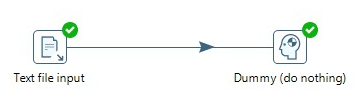
\includegraphics[height=4cm]{imagens/example1.png}
\caption{Dummy}
\label{dummy}
\end{figure}
Após a execução, as métricas de cada step podem ser observadas, a figura \ref{metrics} mostra que o step Text file input escreveu 5 registros e o Dummy leu 5.
\begin{figure}[H]
\centering
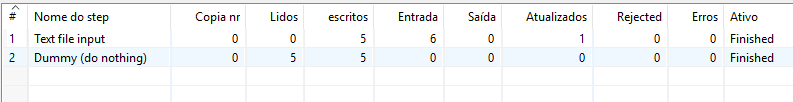
\includegraphics[height=2cm]{imagens/metrics.png}
\caption{Métricas dos steps}
\label{metrics}
\end{figure}
\vfill
\subsubsection{Transform}
Existem diversas transformações que podem ser realizadas nos dados extraídos, como limpeza de campos nulos, geração de novos atributos, formatação de campos. Para isso, o \pdi oferece diversas ferramentas para realizar esse trabalho, como mostra a figura \ref{transformsteps} abaixo.
\begin{figure}[H]
\centering
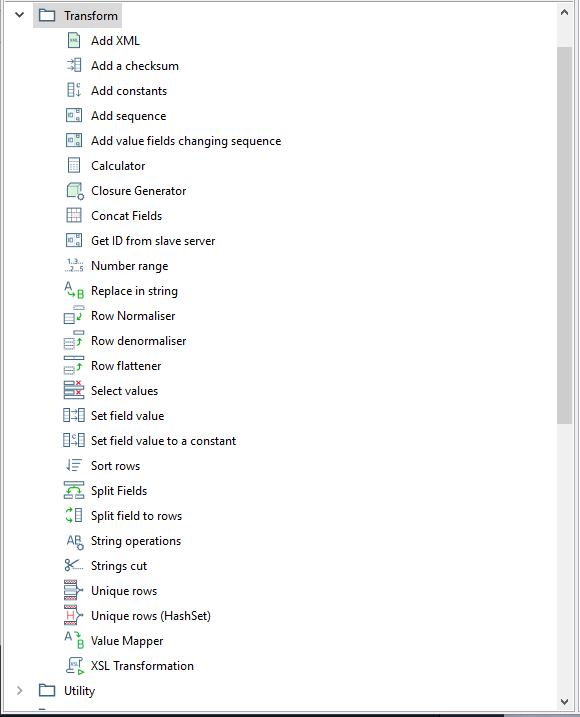
\includegraphics[width=7cm, height=9cm]{imagens/transforms.png}
\caption{Steps da categoria transform}
\label{transformsteps}
\end{figure}
Utilizando os mesmos dados da tabela anterior, novos campos podem ser adicionados, como tempo de vida. Para isso um step da aba \textit{transformation} é utilizado, o \textit{calculator} (\ref{calculator}):
\begin{figure}[H]
\centering
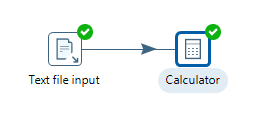
\includegraphics[height=3cm]{imagens/calc.png}
\caption{Step calculator}
\label{calculator}
\end{figure}
Esse step irá calcular o tempo de vida da pessoa utilizando o ano de nascimento e o ano de falecimento, como mostrado na figura \ref{timespan} abaixo:
\begin{figure}[H]
\centering
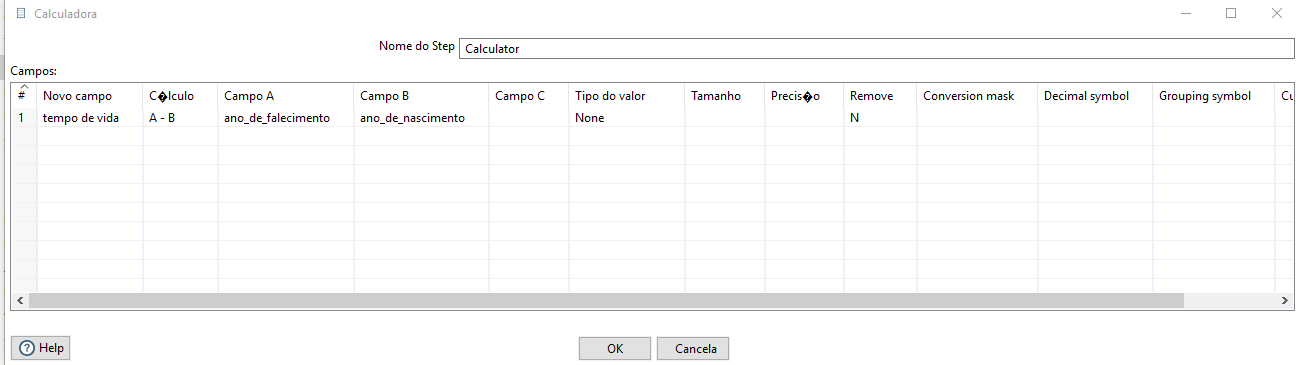
\includegraphics[height=4cm]{imagens/tempovida.png}
\caption{Cálculo do tempo de vida}
\label{timespan}
\end{figure}
A saída desse step pode ser vista no \textit{preview} (figura \ref{preview}):
\begin{figure}[H]
\centering
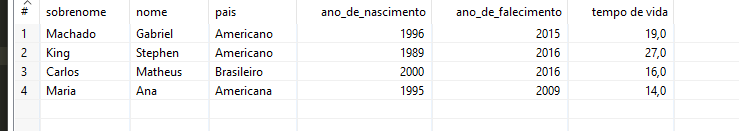
\includegraphics[height=2cm]{imagens/saidavida.png}
\caption{Saída do step}
\label{preview}
\end{figure}
\subsubsection{Load}
A ultima etapa do ETL é o Load (carregamento), o \pdi oferece diversas formas de carregamento, como mostra na figura \ref{outputsteps}.
\begin{figure}[H]
\centering
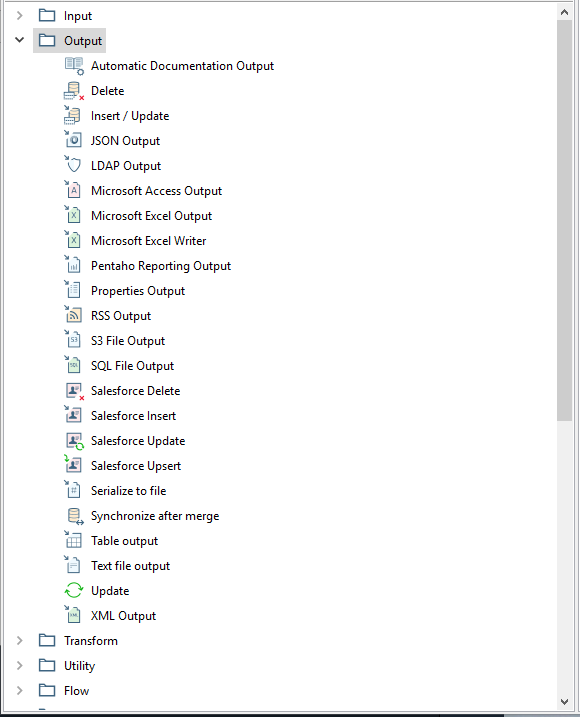
\includegraphics[width=7cm, height=9cm]{imagens/output.png}
\caption{Steps da categoria output}
\label{outputsteps}
\end{figure}
Usando os dados gerados na etapa de transformação, os dados serão carregados em uma tabela no banco de dados, para isso é necessário definir uma conexão no Pentaho e usar o step \textit{Table output}, como mostra a figura \ref{outputstep} abaixo.
\begin{figure}[H]
\centering
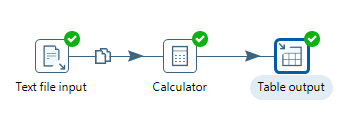
\includegraphics[height=2cm]{imagens/tableoutput.png}
\caption{Saída no banco de dados}
\label{outputstep}
\end{figure}
Na aba \textit{view}, na figura \ref{database}, existe uma opção \textit{connections} e lá tem como criar uma conexão com a base de dados escolhida, nesse caso é o postgres.\\
\begin{figure}[H]
\centering
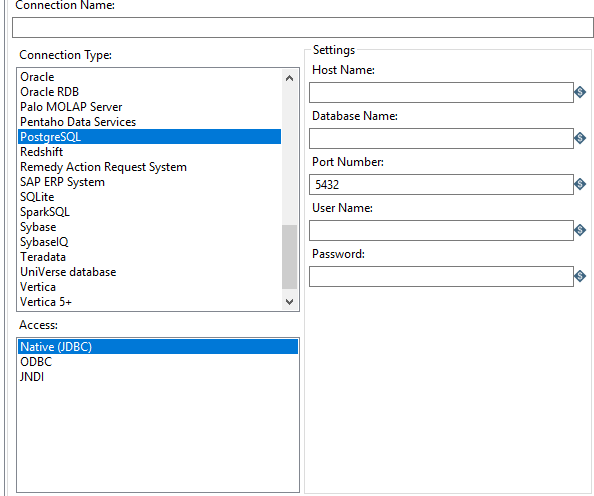
\includegraphics[height=7cm]{imagens/conexao.png}
\caption{Conexões disponíveis no \pdi}
\label{database}
\end{figure}
Quando a conexão for definida, é necessário criar utilizar o step table output (figura \ref{outputtable}), realizando o mapeamento adequado dos campos para serem inseridos na tabela.
\begin{figure}[H]
\centering
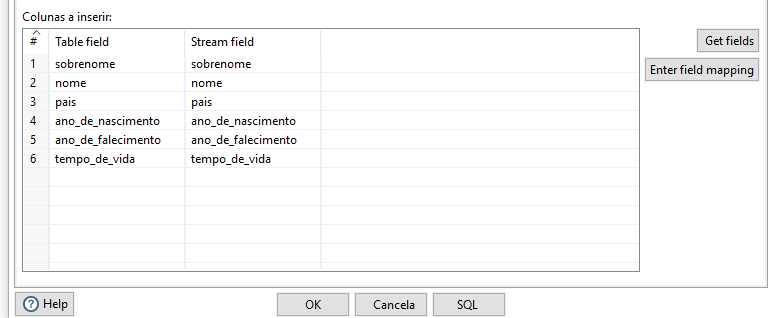
\includegraphics[height=3cm]{imagens/tablemapping.png}
\caption{Mapeamento entre os campos gerados e os campos da tabela}
\label{outputtable}
\end{figure}
Ao executar a transformação, os dados serão carregados na tabela, como mostra a figura \ref{table}.
\begin{figure}[H]
\centering
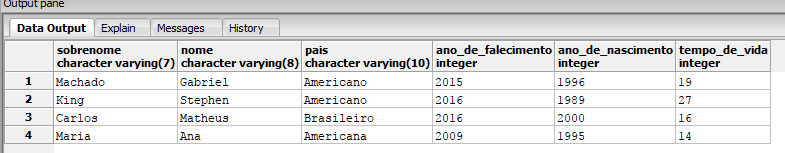
\includegraphics[height=2.5cm]{imagens/saidasql.png}
\caption{Saída no banco de dados}
\label{table}
\end{figure}

\section{Mineração de Dados}

\citeAuthorPageYear{jmj} dizem que o termo mineração de dados poderia ter sido chamado de mineração de conhecimentos dos dados, já que minerar é um processo para encontrar pequenas quantidades de preciosidades de uma grande quantidade de material bruto. 

Outros podem falar que mineração de dados é um sinônimo de KDD (knowledge discovery from data), descobrimento de conhecimento a partir de dados. A mineração também pode ser vista como um passo essencial no processo de descoberta de conhecimento, como mostra a figura \ref{kdd}. 

\begin{figure}[H]
\centering
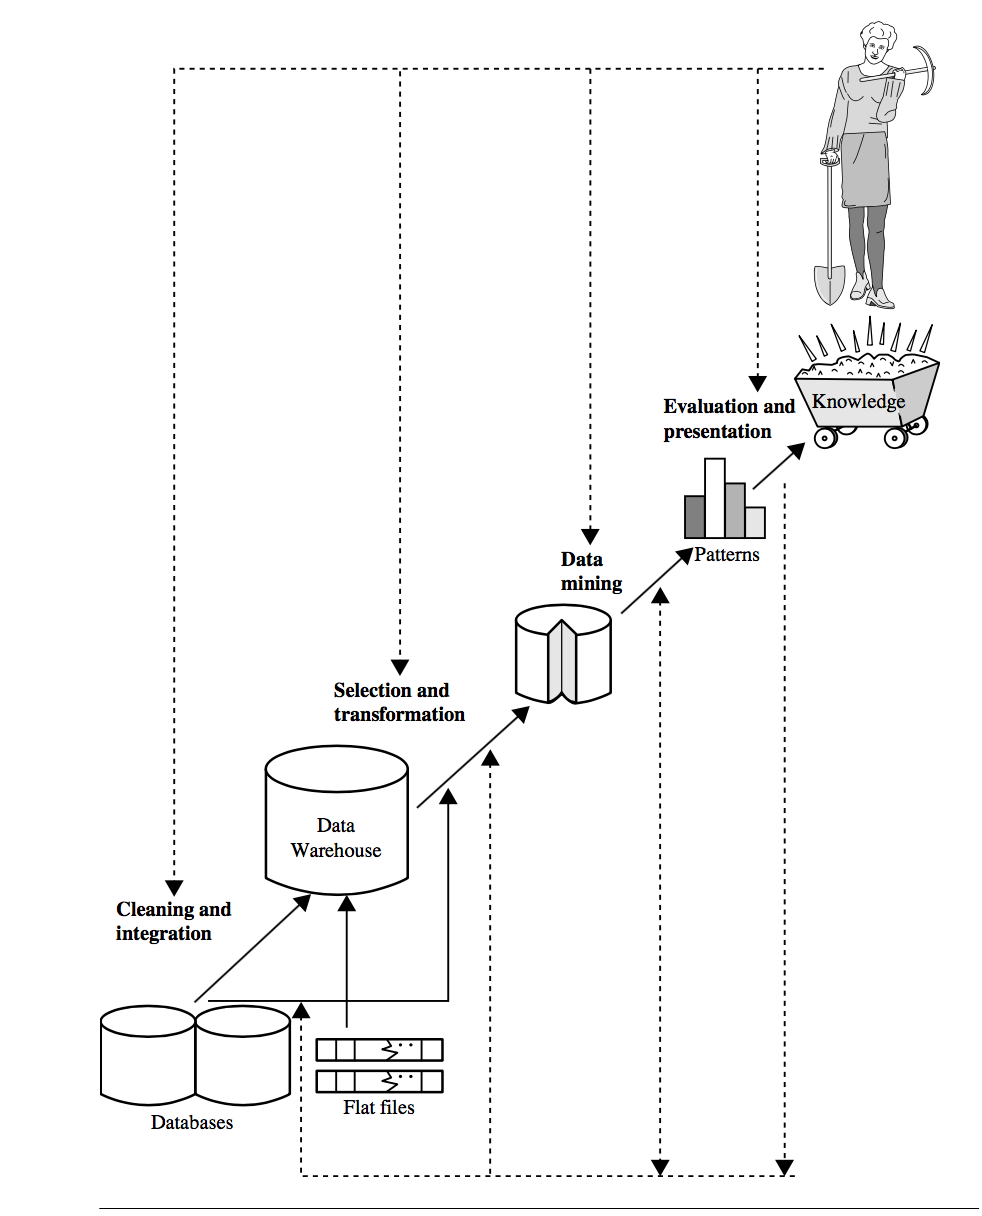
\includegraphics[height=9cm, width=9cm]{imagens/kdd.png}
\caption{Mineração de dados como um processo de descoberta de conhecimento \citep{jmj}}
\label{kdd}
\end{figure}

\citeauthor{jmj} sumarizam mineração de dados em o processo de descobrir padrões interessantes e conhecimento a partir de grandes quantidades de dados. Essas fontes podem ser banco de dados, a internet, data warehouses, dados transacionais, stream de dados, arquivos e etc. 

A mineração de dados tem diversas funcionalidades, como caracterização, que é a sumarização das características gerais de uma classe alvo de dados, discriminação, que é a comparação das características gerais de uma classe alvo com as características de uma ou mais classes diferentes \citep{jmj}. 

Também é usada para encontrar padrões que aparecem frequentemente nos dados. Existem alguns tipos de padrões, como \textit{frequent itemset}, que são itens que geralmente aparecem juntos em um conjunto de dados transacionais, \textit{frequent subsequence} ou \textit{sequencial pattern}, que pode ser o padrão de um cliente que compra primeiro um notebook, depois uma câmera digital e depois um cartão de memória \citep{jmj}. Por último, tem as \textit{frequent substructures}, que, segundo \citeauthor{jmj}, são formas estruturadas que podem aparecer frequentemente, como grafos e árvores, que podem conter \textit{itemsets} e \textit{subsequences}.

Algoritmos de classificação e regressão podem ser usados para analises preditivas, tentando prever dados categóricos ou discretos. A classificação, é o processo de encontrar um modelo que melhor expressa uma classe, esse modelo é derivado da analise de um conjunto de treinamento \citep{jmj}. Os modelos podem ser representados usando árvores de decisão, formulas matemáticas, redes neurais e etc.

Já a regressão, o uso mais comum é para tentar prever valores numéricos contínuos, utilizando algoritmos como regressão linear, regressão lasso e etc.

Também existem os algoritmos de clusterização, que, diferente da classificação e regressão, esse processo analisa os dados sem consultar as suas classes \citep{jmj}. Em alguns casos, os dados podem até vir sem classe. \citeauthor{jmj} dizem que a clusterização pode ser usada para encontrar classes para os grupos de dados. Os clusters são formados de uma forma que os objetos dentro deles tenham uma grande similaridade ao se compararem, mas bem diferentes dos objetos em outros clusters \citep{jmj}.

\subsection{CRISP-DM}
\subsubsection{O que é CRISP-DM}
CRISP-DM, ou Cross-industry standard process for data mining, é uma técnica utilizada no processo de mineração de dados, com uma série de tarefas a serem realizadas para chegar ao melhor resultado.
Segundo \citeAuthorPageYear{dmfd}, mineração de dados não é algo feito uma vez e depois esquecido, o trabalho pode ser aplicado em outros projetos, pode servir de referência
O ciclo de vida da mineração de dados contém seis fases, como apresentado na figura \ref{crispcycle}: entendimento do negócio, entendimento dos dados, preparação dos dados, modelagem, avaliação e implementação. 
A mineração de dados não termina uma vez que a solução é implementada \citep{crispmanual}
\begin{figure}[H]
\centering
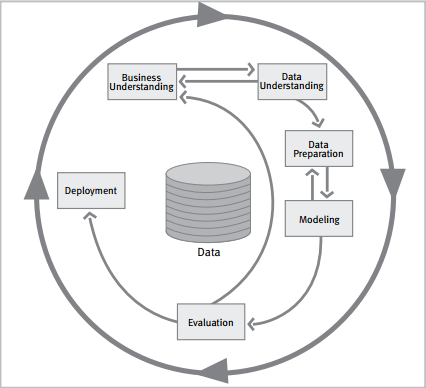
\includegraphics[height=6.2cm]{imagens/lifecycle.png}
\caption{Ciclo de vida (\citeauthor{crispmanual} \citeyear{crispmanual})}
\label{crispcycle}
\end{figure}
Cada uma dessas fases tem diversas tarefas que são realizadas para completar cada uma das fases e cada tarefa tem suas saídas.
\subsubsection{Entendimento do negócio}
A primeira fase do CRISP-DM é o entendimento do negócio, que foca em entender os objetivos do negócio e seus requerimentos de uma perspectiva de negócio.

O primeiro objetivo da analise de dados é entender, sob uma perspectiva de negócio, o que o cliente deseja realizar. Segundo \citeAuthorPageYear{dmfd}, deve ter um entendimento claro do problema que deseja abordar, o objetivo do negócio, as limitações e o impacto. Esse processo produz uma informação da situação do negócio, objetivo do cliente e o critério de sucesso.

Depois é realizada uma avaliação da situação, essa tarefa consiste em um detalhamento maior dos recursos, limitações, premissas e outros fatores que devem ser considerados ao determinar os objetivos da análise de dados e do plano de projeto \citep{crispmanual}.

Outra etapa é determinar os objetivos da mineração de dados, por exemplo, como "prever quantas pessoas irão visitar uma loja no verão, de acordo com informações dos últimos 2 anos dessa loja".

E então é necessário produzir plano de projeto Descrever o plano desejado para atingir os objetivos da mineração de dados e desse modo, os objetivos do negócio \citep{crispmanual}. Esse processo produz o plano de projeto e avaliações iniciais de ferramentas e técnicas

\subsubsection{Entendimento dos dados}
Segundo \citeAuthorPageYear{dmfd}, na segunda fase do projeto de mineração de dados, os dados tem que ser obtidos e tem que verificar se eles são apropriados para as necessidades.

A primeira tarefa dessa fase é coletar dados iniciais e então realizar, caso necessário, o carregamento dos dados em alguma ferramenta. Nessa tarefa é produzida uma lista de todos os datasets adquiridos, junto com localizações, métodos utilizados para coleta e problemas encontrados.

Depois, é feito a descrição dos dados, exploração usando técnicas de visualização. Essa análise pode estar diretamente ligada aos objetivos da mineração de dados \citep{crispmanual}. Essa tarefa produz um relatório da exploração de dados, contendo descobertas iniciais ou hipóteses, e o seu impacto no restante do projeto \citep{crispmanual}.

Depois, é necessário verificar a qualidade dos dados, respondendo perguntas como "os dados estão completos?", "existem valores faltantes?". É criado um relatório da qualidade de dados, com uma lista de problemas encontrados e suas soluções.

\subsubsection{Preparação dos Dados}
A maior parte do tempo gasto no processo de mineração de dados é na preparação deles, já que diversos tratamentos precisam ser feitos nos dados e isso nem sempre é tão simples. A maior parte dos dados usados para mineração foram originalmente coletados e preservados para outros objetivos e precisa ser refinado antes de ser ficar pronto para a modelagem \citep{dmfd}.

Essa fase tem duas saídas, antes das tarefas, que são: \textbf{datasets}, que são os dados produzidos nessa fase e serão usados para modelagem e \textbf{descrição do dataset} \citep{crispmanual}.

A primeira tarefa é \textbf{selecionar os dados} que serão usados na modelagem, baseado nos objetivos da mineração de dados, qualidade e limites técnicos \citep{crispmanual}. É criada uma lista de dados que foram incluídos e excluídos e a razão para isso.

Depois é feita uma \textbf{limpeza dos dados}, que eleva a qualidade dos dados para o nível requerido pelas técnicas de analise selecionadas \citep{crispmanual}. Segundo \citeAuthorPageYear{dmfd}, dificilmente os dados selecionados estarão perfeitamente limpos, mudanças precisarão ser feitas nos dados para atingir o nível necessário. \citeAuthorPageYear{crispmanual} dizem que transformações nos dados podem ser feitas para limpeza e possível impacto na análise de resultados. Nessa etapa é criado um relatório de limpeza de dados: que descreve as ações tomadas para lidar com os problemas encontrados anteriormente.

A tarefa seguinte é \textbf{Construir dados}, essa tarefa consiste na criação de novos campos, dados agregados, ou novos formatos de dados. É produzida uma lista de atributos criados a partir dos atributos existentes e explicar como e por que eles foram criados e uma lista de registros criados, junto com o motivo e como eles foram criados.

A próxima tarefa é \textbf{integrar dados}, já que eles podem estar em diferentes datasets e é necessário a integração desses dados para a fase de modelagem.A saída dessa fase é: \textbf{dados fundidos}: fundir tabelas se refere a juntar duas ou mais tabelas que tem diferentes informações sobre o mesmo objeto \citep{crispmanual}. 

Por último, é necessário \textbf{formatar dados}. Dados frequentemente vem em formatos que não são os convencionais para modelagem \citep{dmfd}, então conversões precisam ser feitas. \citeAuthorPageYear{dmfd} afirma que a fase de preparação de dados deve ser finalizada com um dataset pronto para modelagem e um relatório descrevendo o dataset.

A saída é dados reformatados, convertidos para alguma unidade de medida única para todos os dados (como quilos, em peso).

\subsubsection{Modelagem}
É a fase onde alguma técnica de aprendizado de máquina é utilizada, testada e avaliada para encontrar padrões nos dados, como K-nearest neighbors, Decision Tree e etc.

O primeiro passo da modelagem é \textbf{selecionar a técnica de modelagem} que será usada, caso múltiplas técnicas sejam aplicadas, é necessário executar essa tarefa para cada uma delas \citep{crispmanual}. Nem todas as técnicas de modelagem serão uteis para as necessidades do negócio.

Depois é necessário \textbf{gerar o teste de design}, ou seja gerar procedimentos ou mecanismos para testar a qualidade e validade do modelo \citep{crispmanual}. Os dados geralmente são separados em dois conjuntos, o conjunto de treinamento e o conjunto de teste. O conjunto de treinamento é usado para construir o modelo e o de teste para validar ele. Nessa etapa é gerado descrito como planeja, treina, testa e avalia o modelo.

Depois, é a fase de \textbf{construir o modelo}, Rodar a ferramenta de modelagem para criar um ou mais modelos \citep{crispmanual}. Esse processo produz um documento com as configurações de parâmetros usados, modelos produzidos pela ferramenta e uma descrição dos modelos.

Por fim, é a fase de \textbf{avaliar o modelo}, que sumariza os dados e ranqueia os modelos utilizados e também revisa as configurações dos parâmetros utilizados para tentar reajusta-los até encontrar a melhor possível.

\subsubsection{Avaliação}
Avaliar todo o processo, não só os modelos mas também o processo utilizado para a sua criação.

A primeira tarefa é \textbf{avaliar resultados}. Essa tarefa avalia o grau em que o modelo se adequa ao objetivo original do negócio e busca determinar se existe alguma razão para o modelo estar deficiente.

Essa tarefa avalia o resultado da mineração de dados a respeito do critério de sucesso do negócio, \citeAuthorPageYear{dmfd} afirma que essa tarefa serve para dizer se o projeto atingiu ou não os objetivos definidos no início e seleciona os modelos que atingiram o critério selecionado.

Depois é feita uma \textbf{revisão do processo}, nesse ponto, os modelos resultantes aparentam ser satisfatórios para a necessidade do negócio \citep{crispmanual}. Essa é uma fase usada para rever o processo, como algum problema que foi negligenciado. \citeAuthorPageYear{crispmanual} dizem que se deve sumarizar a revisão e ressaltar as atividades que não foram realizadas e aquelas que devem ser repetidas.

A última fase é \textbf{determinar próximos passos}. A fase de avaliação é concluída com as recomendações para o próximo passo \citep{dmfd}. Decidir se deve finalizar o projeto ou continuar o desenvolvimento. Essa fase também inclui a análise das despesas  e recursos restantes, que podem influenciar na decisão \citep{crispmanual}.
Essa fase produz uma lista de possíveis ações e a decisão.

\subsubsection{Implementação}
O objetivo dessa fase final é a implementação do modelo.
A primeira fase é o plano de implementação, essa fase usa os resultados da avaliação e determina a estratégia de implementação \citep{crispmanual}. 

Ela produz um plano de implementação que sumarizar as estratégias para implementação, os passos necessários e como realizar.
Depois é feito um \textbf{Plano de monitoramento e manutenção}, segundo \citeAuthorPageYear{dmfd}, mineração de dados é um ciclo, então é necessário continuar envolvido com os modelos enquanto eles são integrados ao dia-a-dia. A preparação cuidadosa das estratégias de manutenção ajuda a evitar longos períodos desnecessários de uso incorreto dos resultados da mineração \citep{crispmanual}.

Ela produz um plano de monitoramento e manutenção que sumarizar todas as estratégias de manutenção e monitoramento, incluindo os passos necessários para realiza-los \citep{crispmanual}.
Em seguida, é feito um \textbf{Relatório Final}, que pode ser somente um sumário do projeto e das experiências ou uma apresentação final e compreensível dos resultados da mineração \citep{crispmanual}.
Essa fase produzo relatório final, que sumariza todo o projeto ao juntar todos os relatórios criados até o momento \citep{dmfd} e apresentação final encontro realizado na conclusão do projeto com seu cliente.

Por último, é feita uma \textbf{revisão do projeto} onde o time se reúne e discute o que deu certo e o que não deu, o que pode ser feito novamente e o que não pode e o que deve ser evitado \citep{dmfd}.
A saída é uma documentação de experiência que sumarizar a experiência ganha com o projeto, como erros e acertos, dicas de como selecionar os melhores modelos para situações semelhantes e etc.

\subsection{WEKA}

O WEKA, Waikato Environment for Knowledge Analysis, é uma coleção de algoritmos de aprendizado de máquina e de ferramentas de preprocessamento de dados \citep{weka}. Ele é criado de uma forma que os algoritmos possam ser testados rapidamente nos datasets, ele também contém suporte de mineração de dados, como preparação dos dados, avaliar modelos estatisticamente, visualização dos dados e resultados da aprendizagem. Todas essas ferramentas podem ser acessadas por uma interface simples. O WEKA é escrito em Java e é distribuído sob a GNU General Public License, ele roda em quase toda plataforma e já foi testado nos sistemas operacionnais Linux, Windows e Macintosh \citep{weka}.

\citeAuthorPageYear{weka} dizem que o WEKA contém métodos os principais problemas de mineração de dados, como regressão, clusterização, mineração de regras de associação e seleção de atributos. Conhecer os dados é uma parte integral do trabalho. Uma das formas de utilizar o WEKA é aplicando um método aos dados e analisar a saída para aprender mais sobre os dados \citep{weka}, outra é utilizando modelos para gerar previsões em novas instancias. Uma terceira forma é aplicar diferentes algoritmos e comparar as performances para poder selecionar um para previsão \citeAuthorPageYear{weka}. Uma terceira forma é usar diferentes algoritmos de aprendizado e comparar seus resultados para selecionar um para fazer a previsão. \citeAuthorPageYear{weka} dizem que a implementação de algoritmos de aprendizado é um dos recursos mais valiosos que o WEKA fornece, enquanto os métodos de preprocessamento, também chamados de \textit{filters}, vem logo em seguida. 

\citeAuthorPageYear{weka} dizem que o WEKA pode ser facilmente usado através de uma interface gráfica chamada de \textit{Explorer}. Por exemplo, um dataset pode ser facilmente carregado e construir uma árvore de decisão em cima dele. O WEKA também tem outras interfaces, como o \textit{Knowledge Flow}, que permite processar dados via streaming e o \textit{Experimenter}, que permite responder uma pergunta bem básica e pratica: quais métodos e valores de parâmetros funcionam melhor para determinado problema? O WEKA pode fornecer um ambiente que permite usuários do WEKA comparar uma variedade de algoritmos de aprendizado. \citeAuthorPageYear{weka} dizem que é possível fazer isso interativamente usando a  interface Explorer, mas o Experimenter permite automatizar o processo deixando mais fácil de de rodar classificadores e filtros em um dataset, para coletar estatísticas de performance.

Além disso, todas essas opções podem ser acessadas através de uma interface de linha de comando.

\subsection{Explorer}
A interface gráfica principal do WEKA é a Explorer. Diversas operações podem ser feitas nessa interface.

\subsubsection{Carregando os dados}
Ao abrir o WEKA, deve se selecionar a opção explorer, como mostra na figura \ref{explorer}:

\begin{figure}[H]
\centering

\includegraphics[height=5cm]{imagens/wekaprincipal.png}
\caption{Interface principal do WEKA}
\label{explorer}
\end{figure}

Ao abrir o explorer, a tela deverá exibir diversas opções para carregamento de dados. O formato principal do WEKA é o ARFF, porém ele também é capaz de ler outros formatos, como csv.

\begin{figure}[H]
\centering
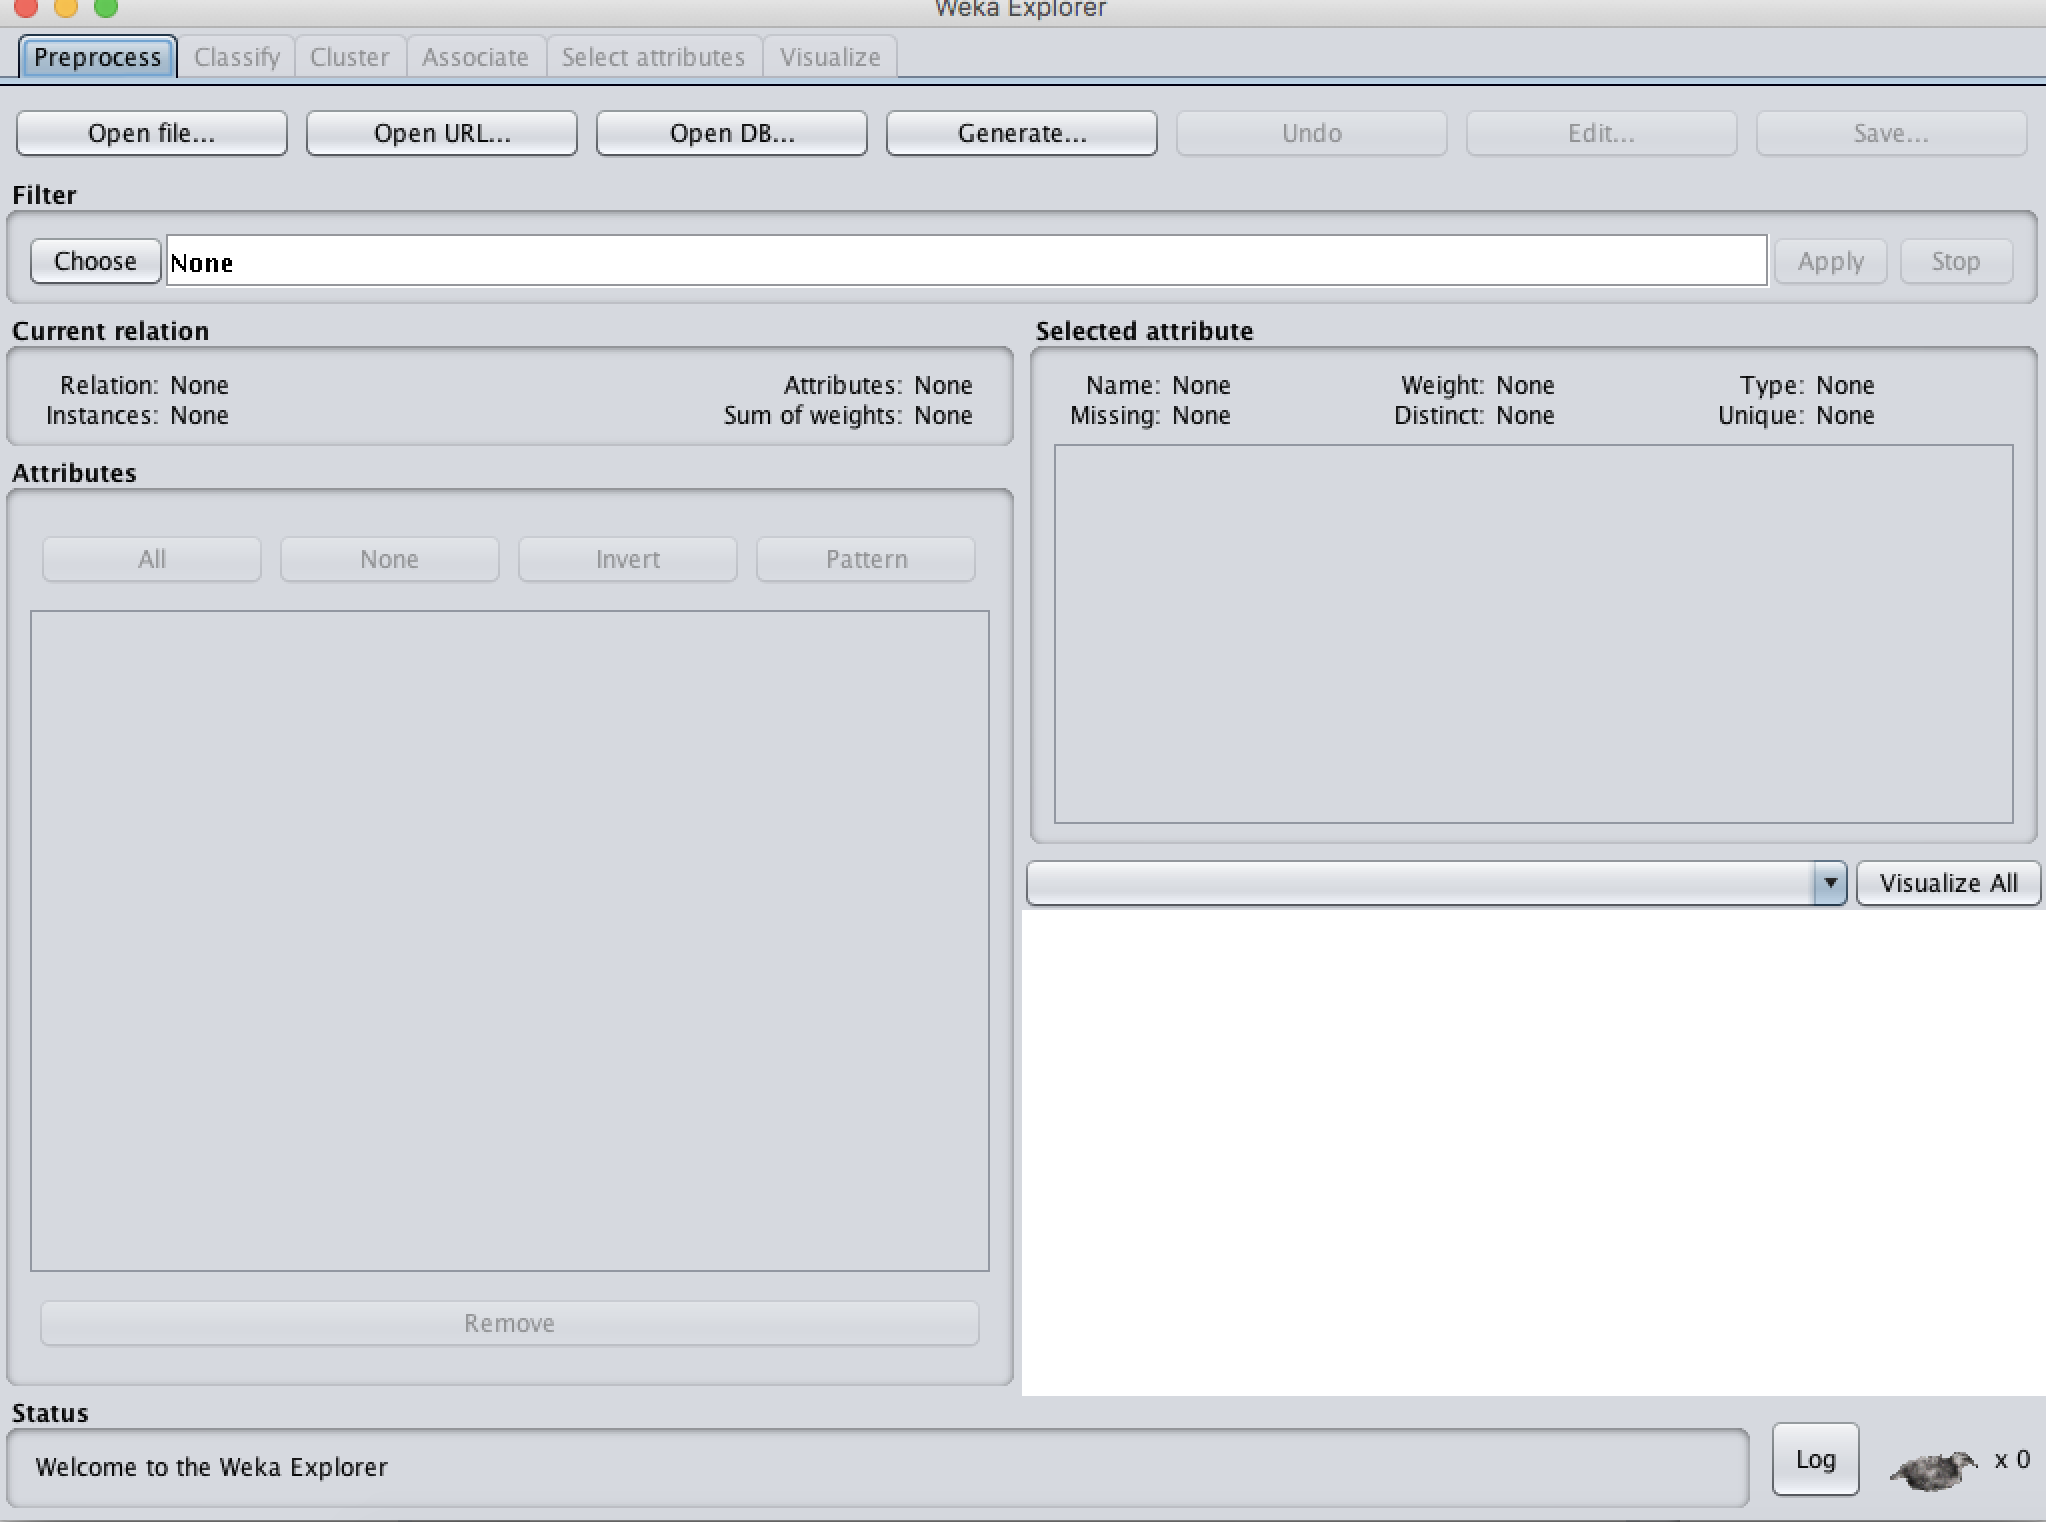
\includegraphics[height=7cm]{imagens/wekapreprocessempty.png}
\caption{Tela de preprocessamento}
\label{figura19}
\end{figure}

Ao carregar os dados, informações sobre cada um dos atributos pode ser encontrada no canto inferior direito e todos os atributos estarão listados no canto esquerdo, como mostra a figura \ref{loadeddata}. A figura \ref{distribuicao} mostra que é possível obter uma distribuição dos valores de cada um dos atributos disponíveis.

\begin{figure}[H]
\centering
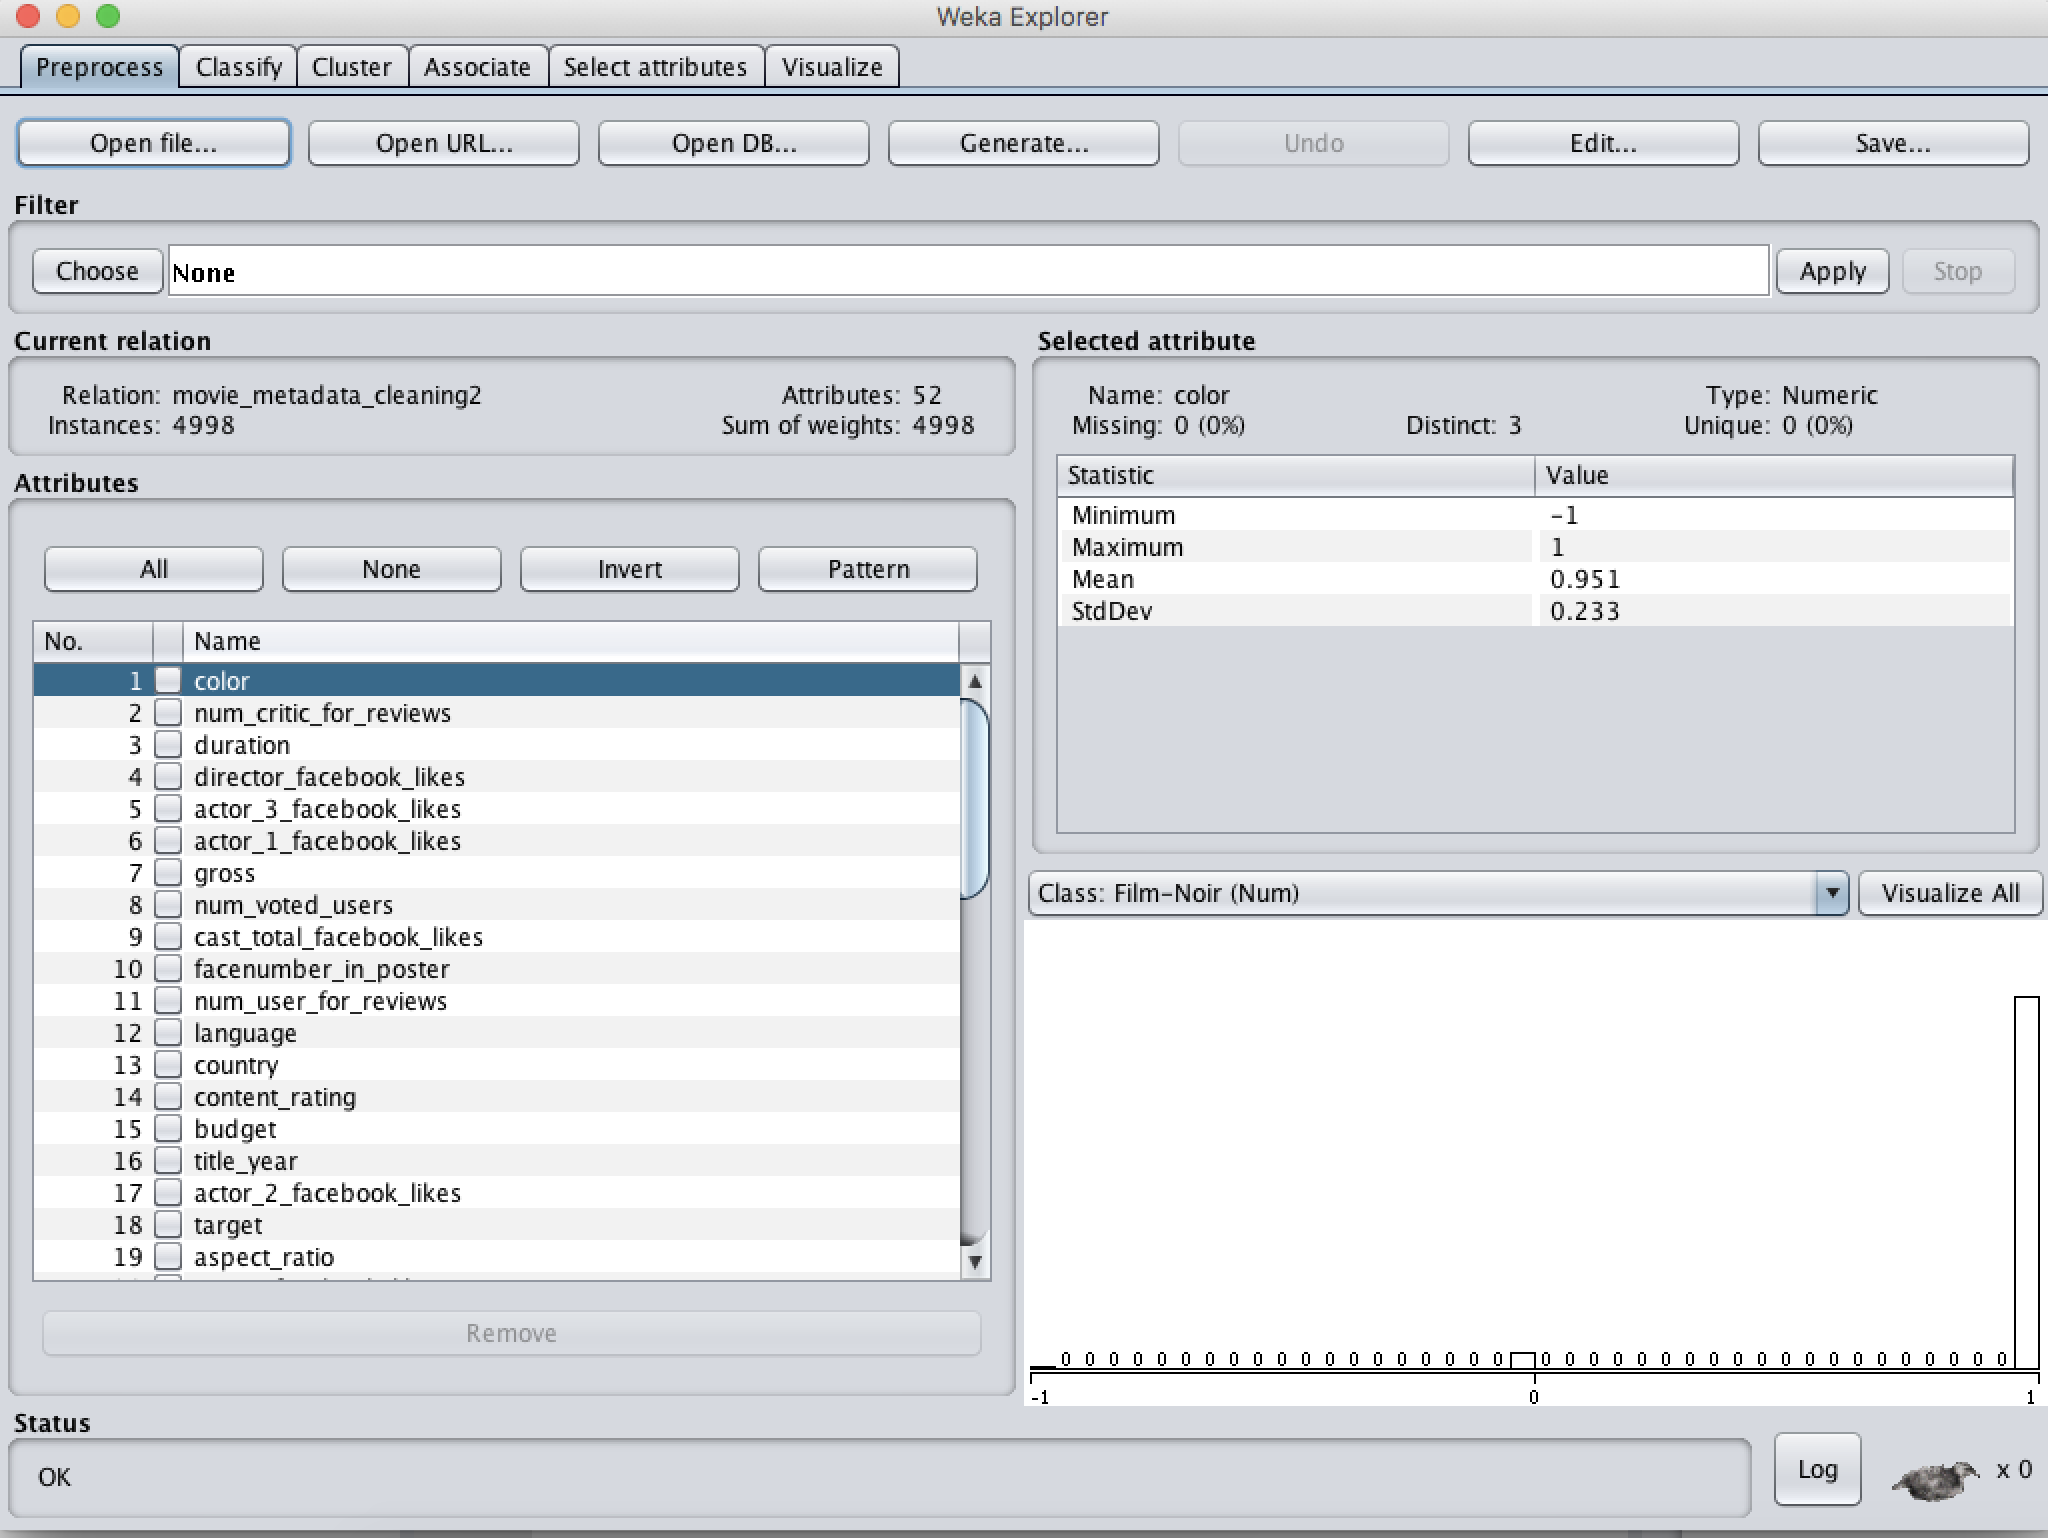
\includegraphics[height=7cm]{imagens/wekapreprocessingfull.png}
\caption{Dados carregados}
\label{loadeddata}
\end{figure}

\begin{figure}[H]
\centering
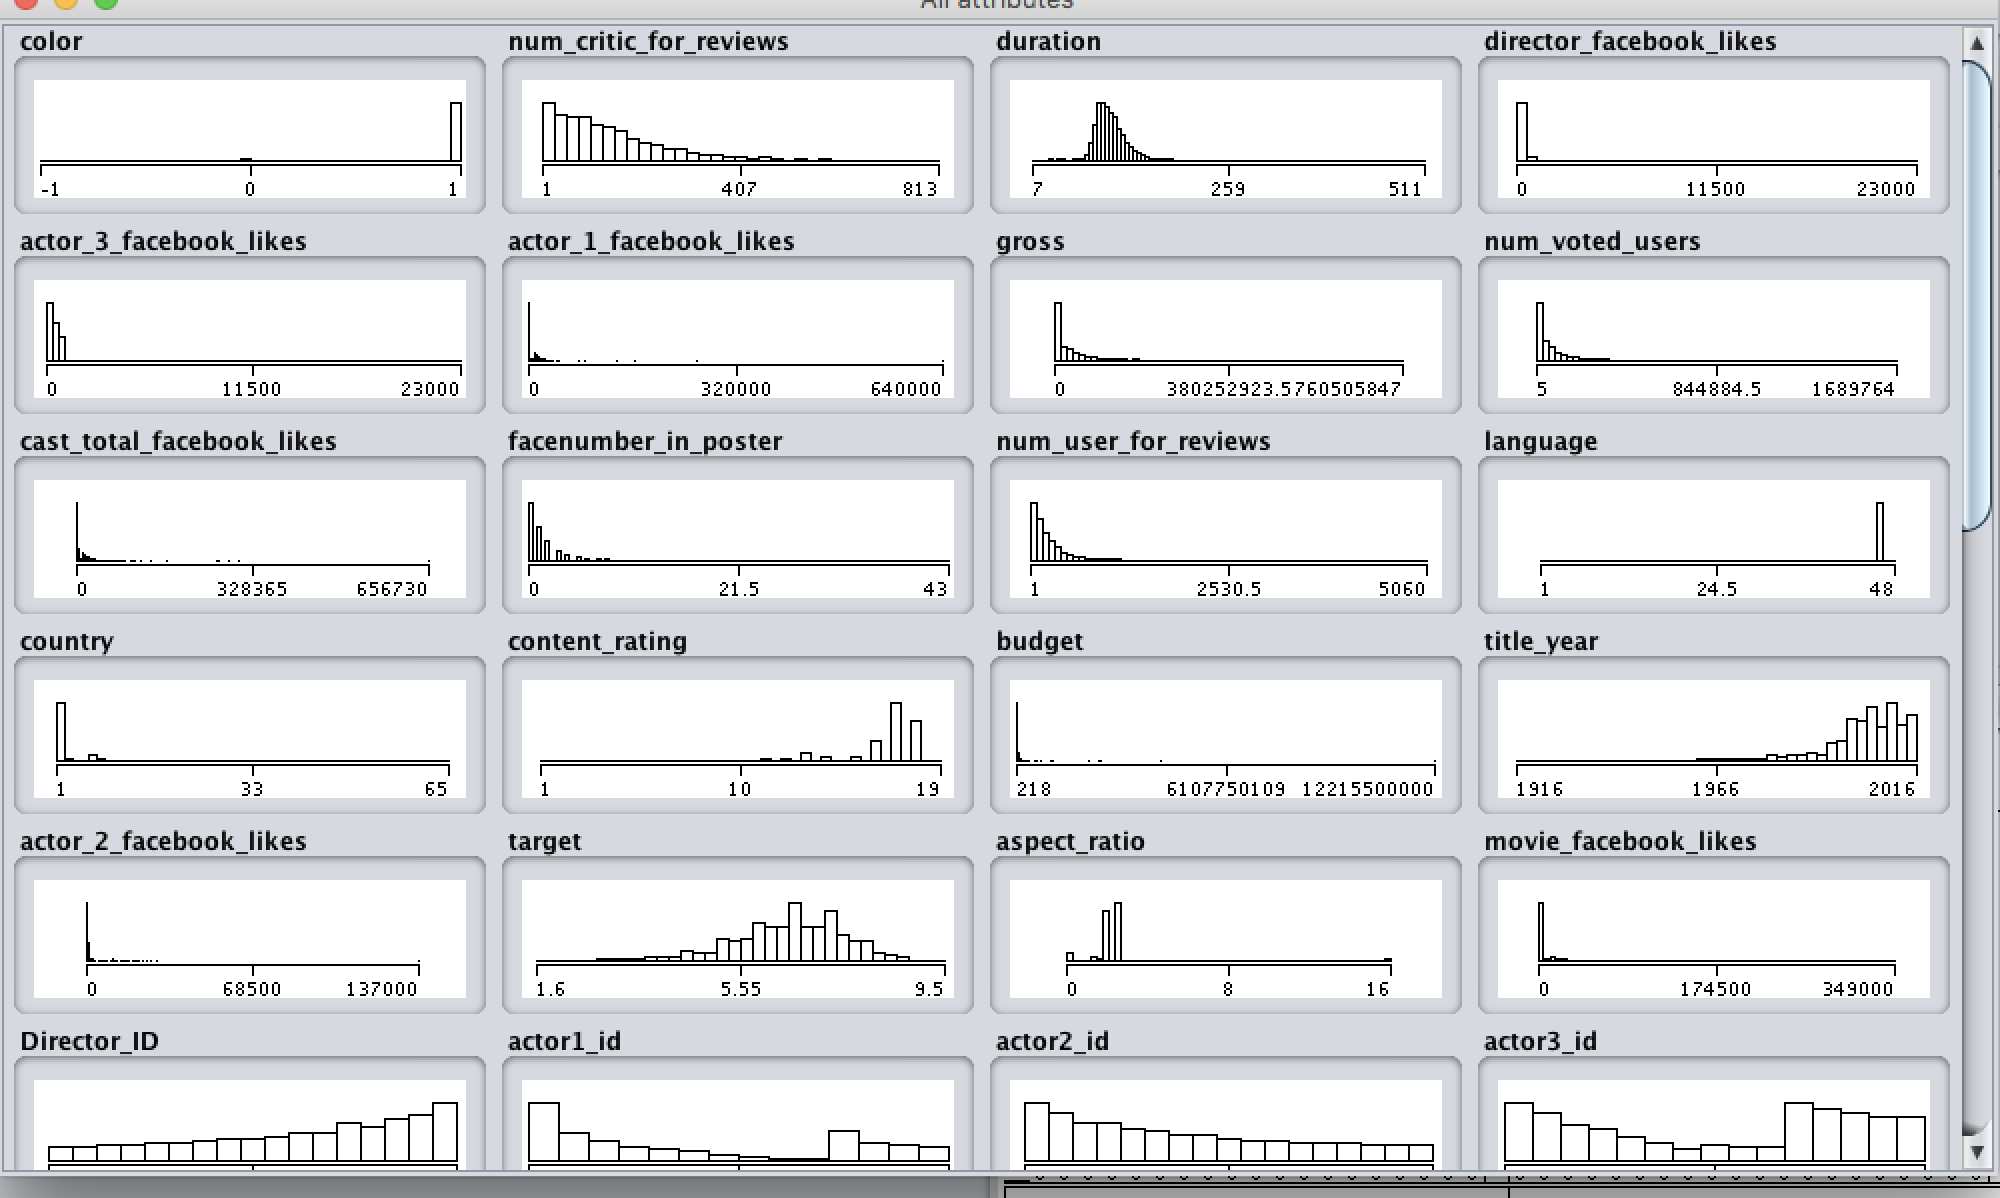
\includegraphics[height=7cm]{imagens/wekadistribuition.png}
\caption{Distribuição dos valores dos dados}
\label{distribuicao}
\end{figure}

Com o WEKA, é possível criar modelos de classificação e de clusterização, nesse caso, foi utilizado o de classificação, como mostra a figura \ref{classificationinterface}. 

\begin{figure}[H]
\centering
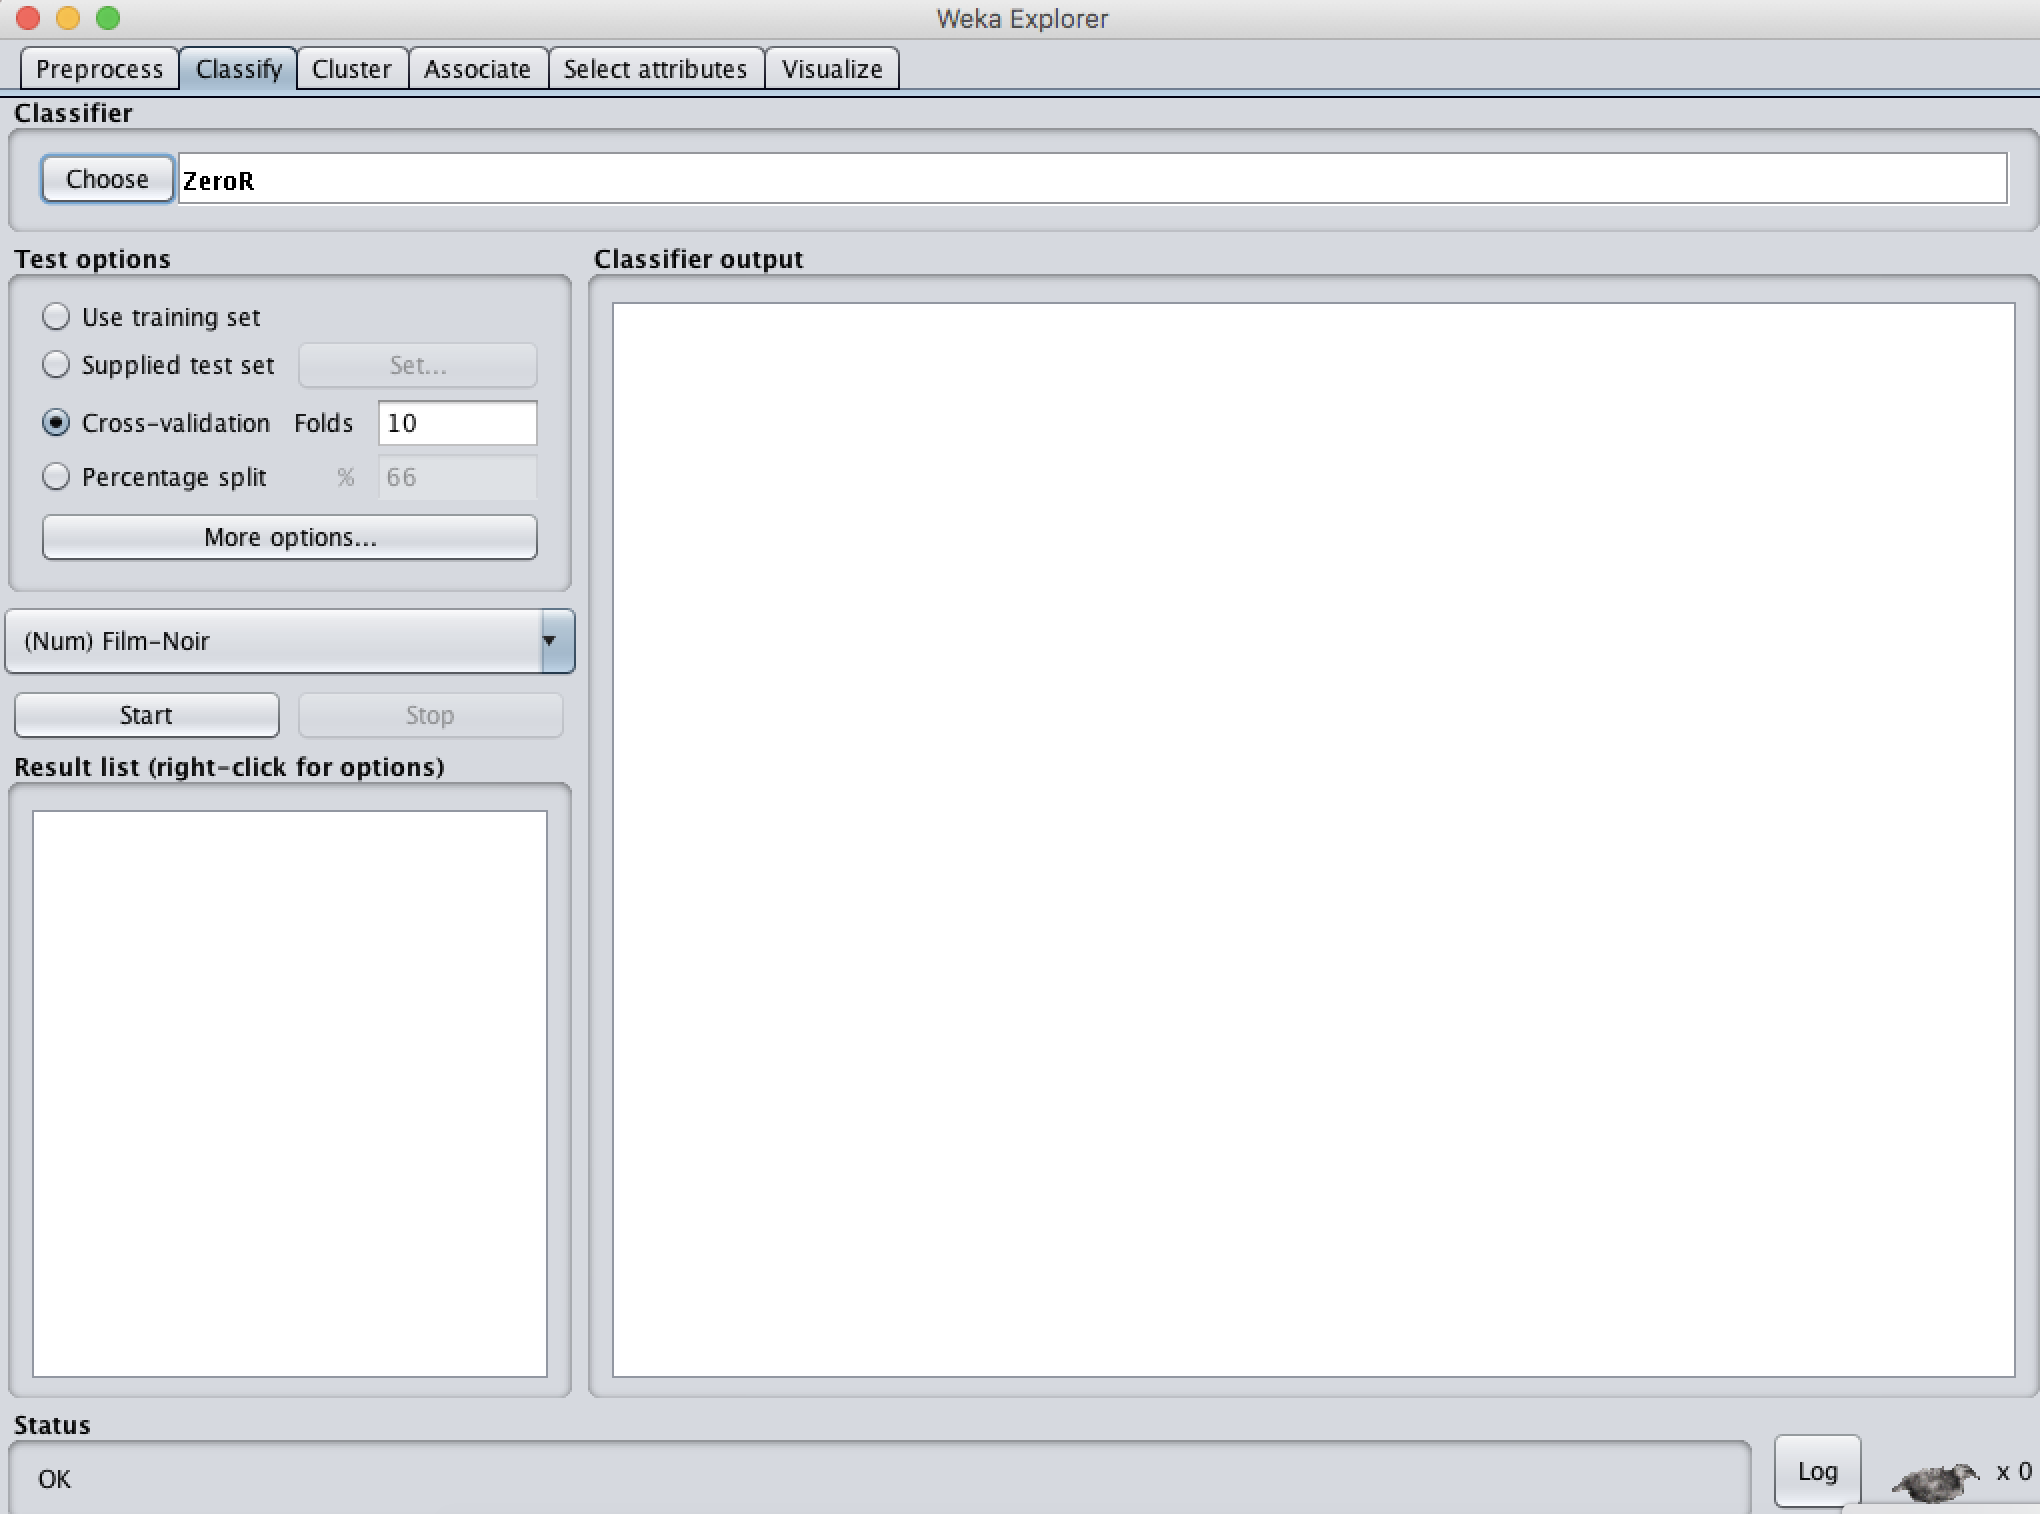
\includegraphics[height=7cm]{imagens/weka.png}
\caption{Interface de classificação}
\label{classificationinterface}
\end{figure}

Ao selecionar um algoritmo de classificação, o campo da direita irá mostrar um log do modelo, junto com o resultado encontrado.
\begin{figure}[H]
\centering
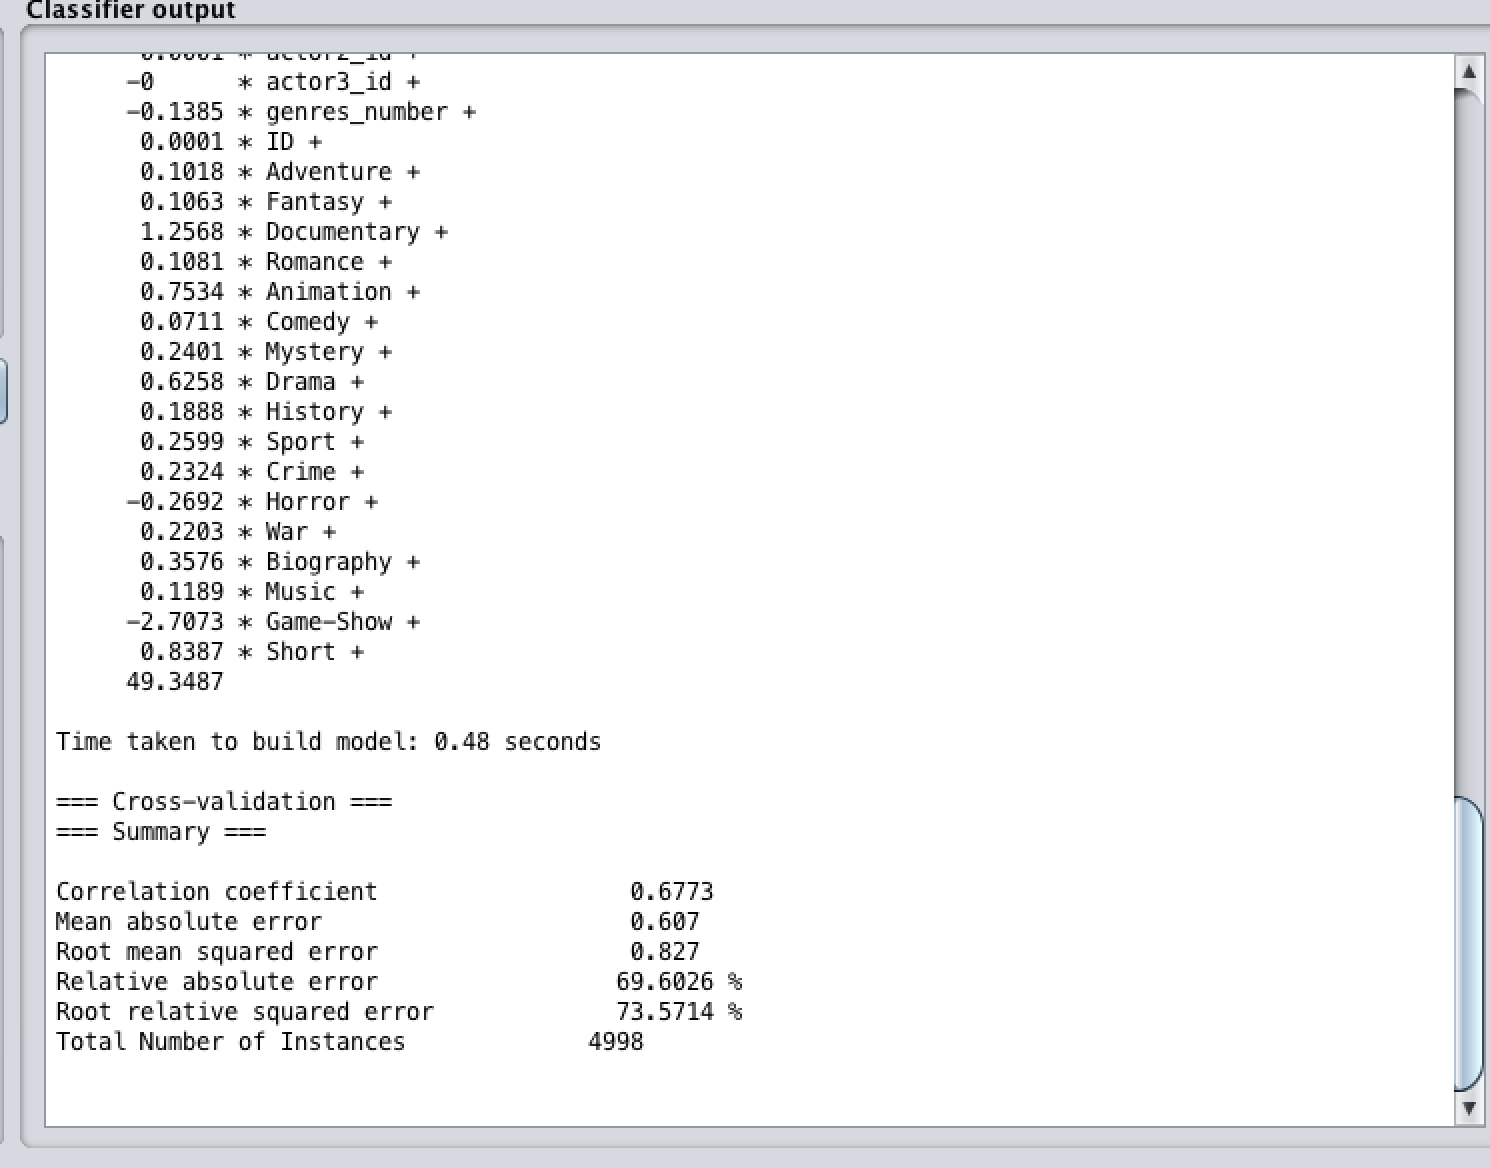
\includegraphics[height=7cm]{imagens/wekauotput.png}
\caption{Dados carregados}
\label{figura23}
\end{figure}
\section{Estudo de Caso}
\subsection{Analise Exploratória}
A tabela 2 contém todas as colunas que existem na base de dados. Um total de 28 colunas numéricas e de texto e 5093 registros. A maioria dos dados tem uma porcentagem de dados faltantes abaixo de 1\%, mas outros, como \textbf{director\_name}, \textbf{plot\_keywords} têm mais de 2\% e a coluna de lucro (\textit{gross}) possui 17.5\%, o que pode atrapalhar um pouco no processo, mas isso ainda não pode ser dito com certeza
\newcolumntype{L}{>{\raggedright\arraybackslash}m{5cm}}
\begin{longtable}{|l|l|L|c|}
\caption{ Colunas do Dataset }
\\ \hline
\textbf{Coluna}              & \textbf{Tipo} & \textbf{Descrição}                      & \textbf{Dados Faltantes} \\ \hline
color                        & String        & Filme é em preto e branco ou colorido   & 0.4\%                    \\ \hline
director\_name               & String        & Nome de quem dirigiu                    & 2.1\%                    \\ \hline
num\_critic\_for\_reviews    & Integer       &                                         & 1\%                      \\ \hline
duration                     & Number        & Duração do filme                        & 0.32\%                   \\ \hline
director\_facebook\_likes    & Number        & Total de likes da pessoa diretora       & 2.1\%                    \\ \hline
actor\_3\_facebook\_likes    & Number        & Total de likes terceira atriz principal & 0.5\%                    \\ \hline
actor\_2\_name               & String        & Nome da segunda atriz principal         & 0.3\%                    \\ \hline
actor\_1\_facebook\_likes    & Number        & Total de likes da primeira atriz        & 0.1\%                    \\ \hline
gross                        & Number        & Lucro do filme                          & 17.5\%                   \\ \hline
genres                       & String        & Gêneros do filme                        & 0\%                      \\ \hline
actor\_1\_name               & String        & Nome da primeira atriz principal        & 0.1\%                    \\ \hline
movie\_title                 & String        & Título do filme                         & 0\%                      \\ \hline
num\_voted\_users            & Integer       & Número de usuários que votaram          & 0\%                      \\ \hline
cast\_total\_facebook\_likes & Integer       & Total de likes do elenco                &                          \\ \hline
actor\_3\_name               & String        & Nome terceira atriz principal           & 0.5\%                    \\ \hline
facenumber\_in\_poster       & Number        & Número de rostos no poster do filme     & 0.3\%                    \\ \hline
plot\_keywords               & String        & Palavras-chave do enredo                & 3\%                      \\ \hline
movie\_imdb\_link            & String        & Link do filme no IMDB                   & 0\%                      \\ \hline
num\_user\_for\_reviews      & Number        & Número de usuários que fizeram review   & 0.4\%                    \\ \hline
language                     & String        & Língua em que o filme foi distribuído   & 0.2\%                    \\ \hline
country                      & String        & País de origem do filme                 & 0.1\%                    \\ \hline
content\_rating              & String        & Classificação indicativa                & 6\%                      \\ \hline
budget                       & Number        & Orçamento                               & 9.8\%                    \\ \hline
title\_year                  & Number        & Ano de lançamento                       & 2.1\%                    \\ \hline
actor\_2\_facebook\_likes    & Number        & Total de likes Segunda atriz principal  & 0.3\%                    \\ \hline
imdb\_score                  & Number        & Nota no IMDB                            & 0\%                      \\ \hline
aspect\_ratio                & Number        & proporção da tela                       & 6.5\%                    \\ \hline
movie\_facebook\_likes       & Number        & Total de likes do filme              & 0\%                      \\ \hline
\end{longtable}


Uma análise foi realizada usando \textbf{python}\footnote{Todos os arquivos gerados podem ser encontrados em \url{https://github.com/gabriel-ma/TCC}} e as bibliotecas \textbf{pandas}\footnote{https://pandas.pydata.org/}, \textbf{matplotlib}\footnote{https://matplotlib.org/} e \textbf{seaborn}\footnote{https://seaborn.pydata.org/}. Inicialmente os dados foram importados e uma análise geral foi realizada com o \textbf{pandas profiling}\footnote{https://github.com/pandas-profiling/pandas-profiling} e observações iniciais foram feitas:
\begin{enumerate}
    \item 15 colunas contém dados numéricos
    \item 12 são dados categóricos
    \item Existem filmes de cerca de 65 países
    \item Existem 45 dados duplicados
    \item O ator que mais participou dos filmes é o Robert De Niro 
    \item A maior parte dos filmes é colorida
    \item 3808  filmes foram feitos nos Estados Unidos
    \item O lucro médio dos filmes foi de \$48.468.000,00
    \item O filme com a maior nota tem 9.5
    \item O filme com a menor nota tem 1.6
    \item A nota média dos filmes é de 6.44
    \item O orçamento médio dos filmes é de \$39.753.000,00
    \item 4662 filmes estão disponíveis em inglês
    \item O filme com o maior número de críticas tem 813 críticas
    \item Com 258, 2009 é o ano com a maior quantidade de filmes nos dados
    \item A coluna \textbf{cast\_total\_facebook\_likes} tem uma correlação muito alta\\ com \textbf{actor\_1\_facebook\_likes}
\end{enumerate}

Uma hipótese que pode logo levantada é de que os dados estão enviesados. De acordo com o item 10, cerca de 3808 filmes foram feitos nos Estados Unidos, fazendo com que ao treinar o modelo a partir desses dados, o algoritmo pode ser ótimo para prever, por exemplo, notas de filmes norte-americanos, mas péssimo para prever filmes sul-americanos.

\begin{figure}[H]
\centering
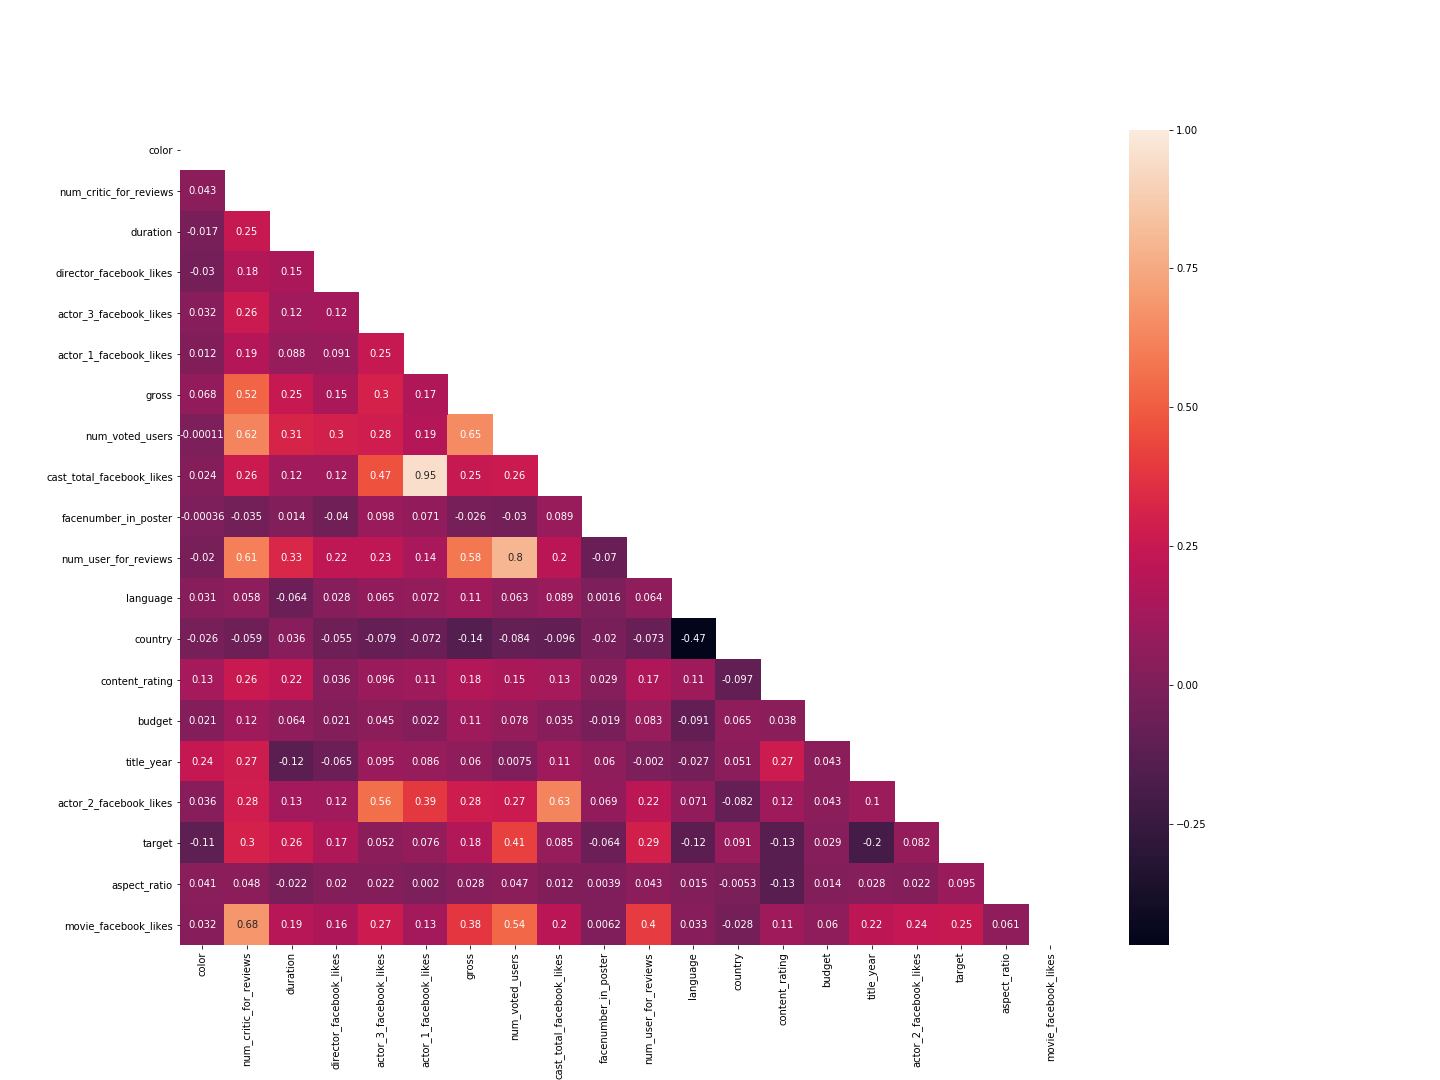
\includegraphics[height=15cm]{imagens/heatmap.png}
\caption{Heatmap}
\label{heatmap}
\end{figure}

A figura \ref{heatmap} representa um \textit{heatmap} (mapa de calor) que mostra o quanto os campos estão correlacionados. Por exemplo, se um campo \textbf{x} tem uma correlação positiva muito alta com o campo \textbf{y}, isso significa que quando o valor de um aumentar, o valor do segundo campo provavelmente também irá aumentar. Na figura acima, é possível notar que quanto maior a relação entre dois campos, mais claro o quadrado que exibe a relação fica no mapa. 
Na mesma figura é possível ver que existem campos com uma correlação maior com a nota (\textit{target}) como \textbf{num\_crit\_for\_reviews} e \textbf{num\_voted\_users}. 

É possível assumir que algumas colunas não são necessárias para a análise, como \textbf{imdb\_link}, que é apenas o \textit{link} do filme na página do IMDB e não tem relação nenhuma com a nota.

Alguns gráficos foram gerados para poder realizar uma análise mais profunda dos dados: 

\begin{figure}[H]
\centering
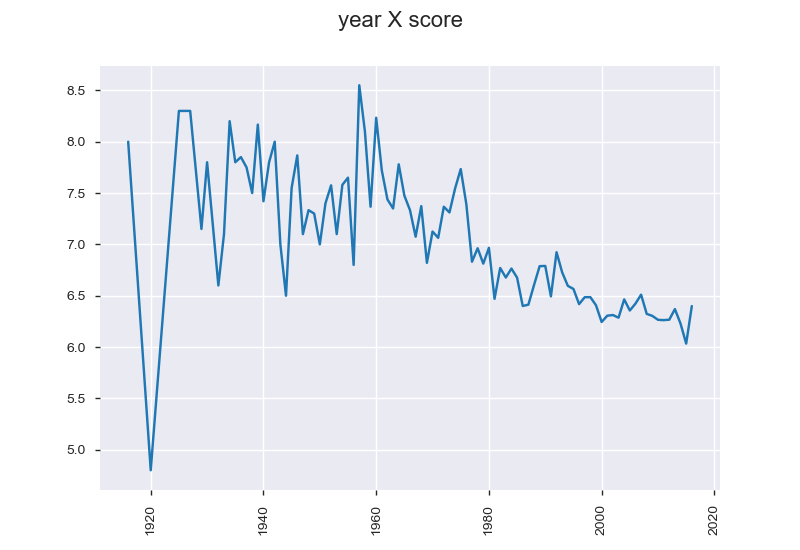
\includegraphics[height=10cm]{imagens/yearXscore.png}
\caption{Ano X Nota}
\label{yearXscore}
\end{figure}

Na figura \ref{yearXscore} é possível perceber que a média das notas veio caindo. Excetuando o ano de 1920, que teve uma média incrivelmente baixa, os anos seguintes se mantiveram entre 8.5 e 6.5. A partir da década de 80, o cenário começou a mudar e as médias começaram a baixar, chegando em 2016 (último ano que existe no \textit{dataset}) a aproximadamente 6.5.

\begin{figure}[H]
\centering
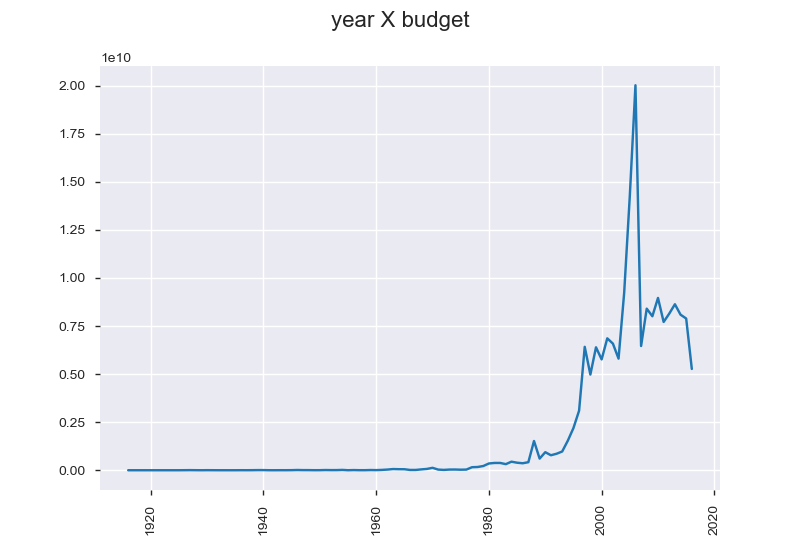
\includegraphics[height=10cm]{imagens/yearXbudget.png}
\caption{Investimento X Ano}
\label{budgetXyear}
\end{figure}
A figura \ref{budgetXyear} acima mostra que o investimento nos filmes aumentou consideravelmente. Entre a década de 90 e os anos 2000 teve um aumento quase exponencial.

\begin{figure}[H]
\centering
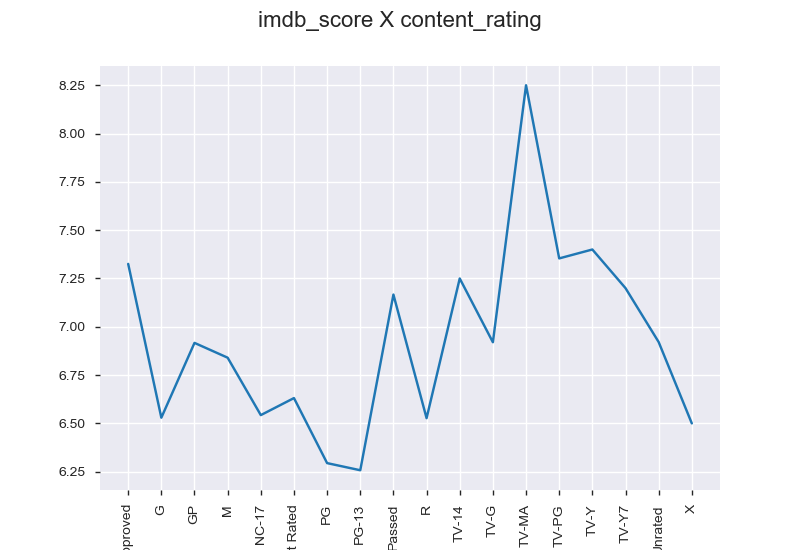
\includegraphics[height=10cm]{imagens/scoreXcontent.png}
\caption{Classificação indicativa X Nota}
\label{ratingXscore}
\end{figure}
Outra variável que pode influenciar a nota dos filmes é a classificação indicativa. A figura \ref{ratingXscore} mostra que filmes com a classificação \textbf{TV-MA} tendem a ter uma nota maior. Cerca de 2098 amostras encontradas nesses dados contêm a classificação \textbf{R}, porém a média das notas para esses filmes é de pouco mais de 6.5.

\subsection{Extract}
No primeiro passo do ETL, que é o de extração, \textit{extract}, os dados foram extraídos utilizando o \pdi com um \textit{step} de \textit{read csv}, já que o arquivo é um csv. Foi preciso formatar corretamente os campos de números, e nos de texto foi necessário realizar uma operação \textit{trim} para remover espaços em brancos desnecessários. 

\subsection{Transform}
No segundo passo do ETL, o de transformação, \textit{transform}, foram usados passos para substituir alguns valores nulos, como, por exemplo, no campo \textbf{color}, os dados que não eram preenchidos eram substituídos por 0. 

Com o auxílio da linguagem \textbf{python} com as bibliotecas \textbf{pandas}, \textbf{sklearn}\footnote{https://scikit-learn.org/stable/} e \textbf{numpy}\footnote{http://www.numpy.org/} através do \textbf{Jupyter Notebook}\footnote{http://jupyter.org/}, foi possível realizar diversos tratamentos adicionais nos dados, como preencher valores nulos, que não foram tratados no \pdi pela média, quando necessário. No \pdi foi adicionado um \textit{step} de \textbf{group by} para tratar campos, substituindo o seu valor (quando faltante) pela média ou pela mediana. 

Outros \textit{steps} foram usados para fazer um mapeamento dos dados, por exemplo, a coluna \textbf{director\_name} do jeito que está originalmente não iria ser muito útil na análise, pois os algoritmos de regressão utilizados não conseguem trabalhar com campos de texto. Para isso, esses dados foram substituídos por números que identificam o diretor do filme. O mesmo aconteceu com as colunas \textbf{color}, \textbf{language}, \textbf{country}, \textbf{content\_rating} e as colunas de atores. Manter essas colunas como texto iria atrapalhar a análise, já que vários dos algoritmos usados não conseguem trabalhar com campos de texto. A figura \ref{pentahoTransformation} mostra todos os \textit{steps} que foram criados para o processo de ETL no \pdi.

\begin{figure}[H]
\centering
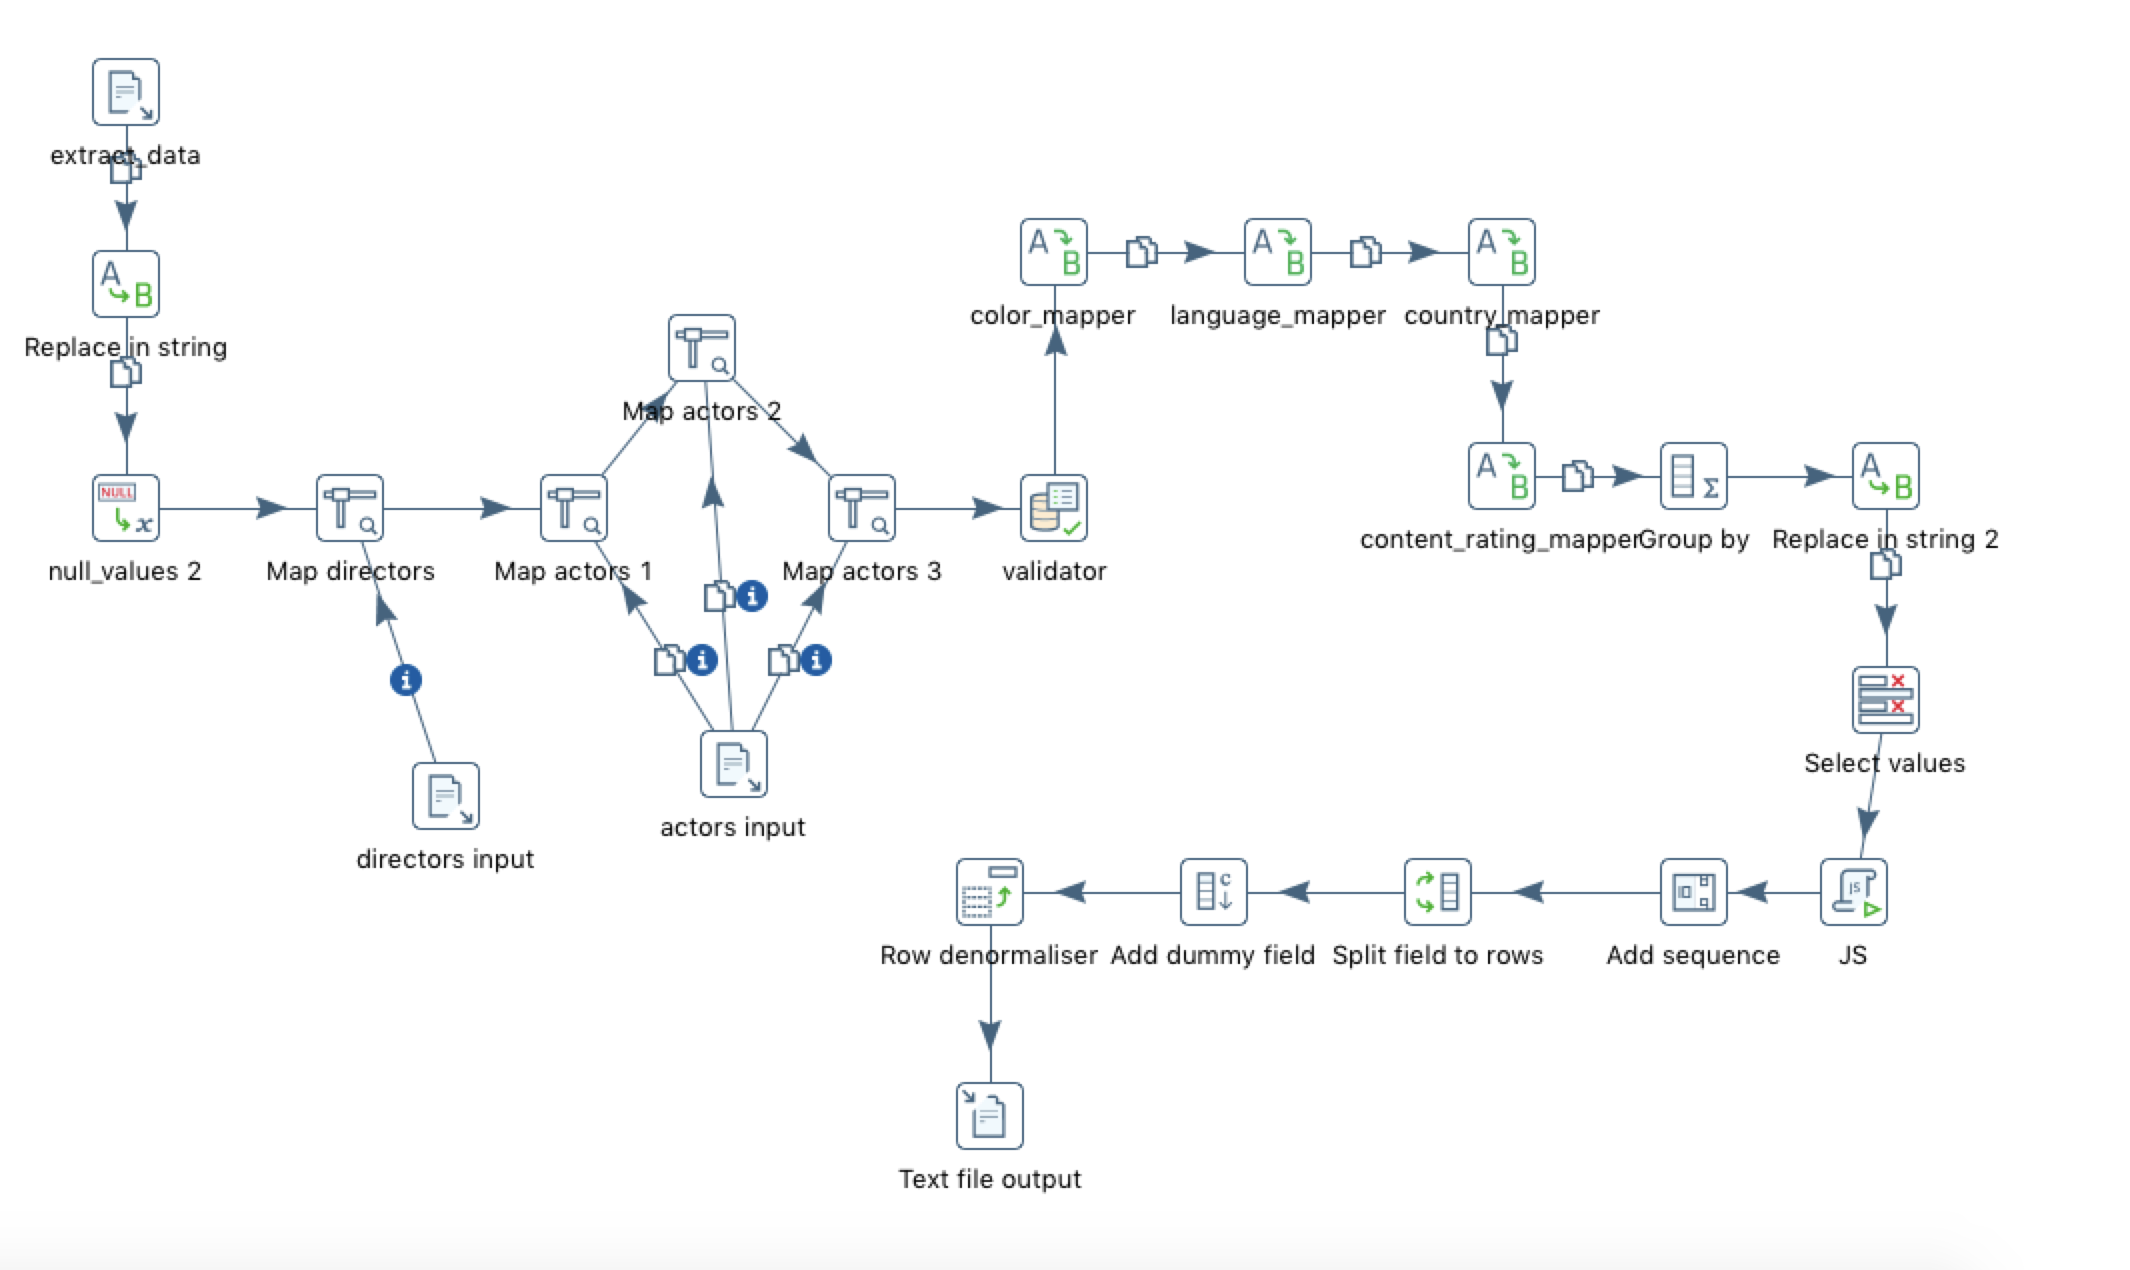
\includegraphics[height=6cm, width=9cm]{imagens/transformacao.png}
\caption{Processo do pentaho}
\label{pentahoTransformation}
\end{figure}

Algumas colunas novas foram geradas e essas são derivadas de colunas existentes, como \textbf{plot\_keywords\_num}. Tiveram \textit{steps} responsáveis por fazer uma transformação na coluna \textbf{genres}, transformando cada valor em uma coluna e se o filme conter o gênero da coluna, ela é marcada com 1, senão, 0, como mostra a figura \ref{newcolumns}.

\begin{figure}[H]
\centering
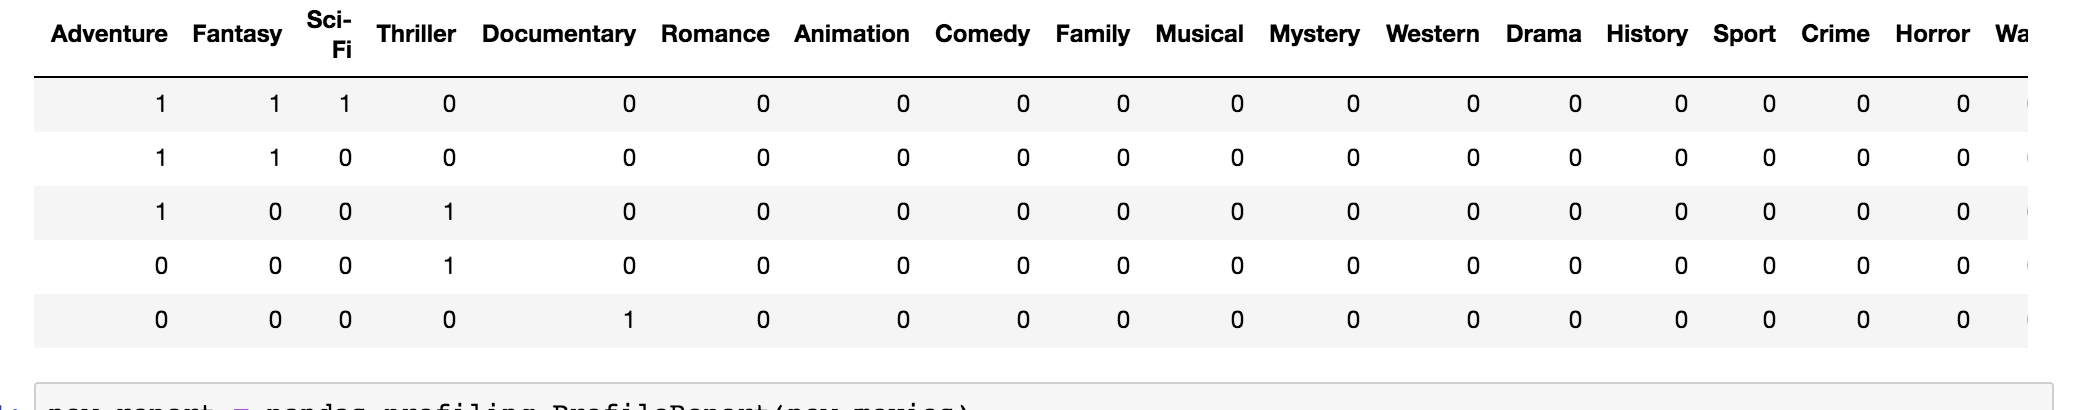
\includegraphics[height=3cm]{imagens/genres.png}
\caption{Novas colunas de gênero}
\label{newcolumns}
\end{figure}

\subsection{Load}
O último passo, que é o carregar, \textit{load}, apenas carregou os dados em um outro arquivo csv, com o \textit{step text file output}. Esse arquivo foi usado mais tarde no WEKA.

\subsection{Hipóteses}
A hipótese principal é se seria possível prever a nota de um filme com base nos dados disponíveis e qual o nível de precisão.

Além disso, como dito anteriormente, outra hipótese que pode ser levantada é a de que os dados estão enviesados, já que contêm muitos filmes feitos nos Estados Unidos. Uma outra que pode ser levada em consideração é se o diretor do filme tem grande influência sobre a nota dele. Também é possível verificar o quanto a nota do filme vai influenciar no lucro dele e o quanto o investimento feito pode influenciar a nota.

Após todos os passos acima, o próximo é realizar o processo de \textit{machine learning}, levando em consideração todos as hipóteses levantadas. Os dados foram carregados no WEKA e algoritmos de aprendizado de máquina foram usados. Um segundo \textit{dataset}, sem os filmes norte-americanos, foi criado e também carregado no WEKA, para validar ou não a afirmação feita de que os dados estão enviesados. 

Em resumo:

\begin{itemize}
    \item Prever nota de um filme com base nos dados disponíveis
    \item A grande quantidade de filmes dos EUA adiciona um viés nos dados
    \item Influência do investimento na nota
    \item Influência do país na nota
    \item Influência do diretor na nota
\end{itemize}

\subsubsection{Resultados}
As análises realizadas levaram em conta o MSE, \textit{mean squared error}, e os valores foram elevados ao quadrado, no caso RMSE, \textit{root mean squared error}, que calcula o quadrado da diferença dos erros, como mostra a formula abaixo:

$RMSE = \sqrt{\frac{1}{n}\Sigma_{i=1}^{n}{\Big({predicted-actual}\Big)^2}}$
 
O MSE é muito usado em vários algoritmos porque ele tende a ser a medida mais fácil de ser manipulada matematicamente.

Em um primeiro momento, os dados gerados a partir do \pdi e as bibliotecas do \textit{python} foram usados para selecionar o algoritmo de predição com os melhores resultados. Para isso, foram realizadas diversas análises com esses algoritmos no WEKA: os que tiveram o menor RMSE, tanto método de \textit{cross-validation} e o de 70\% split, foram \textit{linear regression}, \textit{bagging}, \textit{random committee} e \textit{random forest}, como mostra as tabelas abaixo:

\begin{longtable}{|l|l|l|}
\caption{Resultados da previsão usando \textit{cross-validation}}
\label{cvfull}
\\ \hline
\textbf{Algoritmo} & \textbf{RMSE} & \textbf{Percentual de Erro} \\ \hline
Linear Regression      & 0.827         & 69.6026\%                   \\ \hline
Bagging                & 0.7685        & 63.207\%                    \\ \hline
Random Committee       & 0.7754        & 63.8278\%                     \\ \hline
Random Forest          & 0.7748        & 61.7894\%                     \\ \hline
\end{longtable}


\begin{longtable}{|l|l|l|}
\caption{Resultados da previsão usando 70\% para treinamento e 30\% para teste}
\label{splitfull}
\\\hline
\textbf{Algoritmo} & \textbf{RMSE} & \textbf{Percentual de Erro} \\ \hline
Linear Regression      & 0.8122        & 71.3281\%                   \\ \hline
Bagging                & 0.7529        & 64.2981\%                   \\ \hline
Random Committee       & 0.7468        & 65.3504\%                   \\ \hline
Random Forest          & 0.7245        & 63.0243\%                   \\ \hline
\end{longtable}



Para testar a hipótese de que a grande quantidade de filmes dos EUA adiciona um viés nos dados, os filmes feitos nos Estados Unidos foram removidos do \textit{dataset}. Removendo esses filmes e aplicando o algoritmo que teve os melhores resultados, o \textit{random forest}, ele retornou um erro de 0.7674 (figura \ref{nousacv}) com o método \textit{cross-fold validation} e 0.7341 (figura \ref{nousasplit}) usando o \textit{percentage split}. Os resultados não mudaram tanto, porém a quantidade de amostras sim, foram de 4998 para 1224. Talvez o filme ser do EUA tenha de fato algum tipo de influência, porém não é possível definir com clareza somente com essa quantidade de dados, já que muita informação se perde.

\begin{figure}[H]
\centering
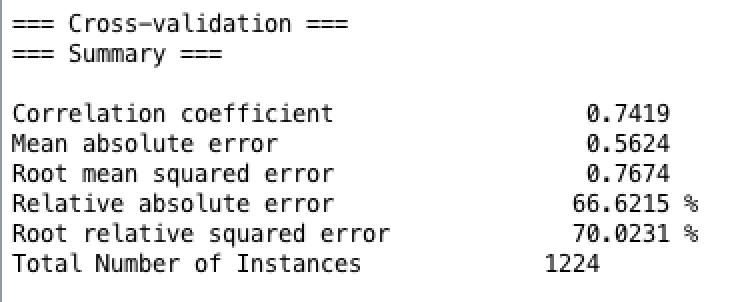
\includegraphics[height=5cm]{imagens/sem_usa_cv.png}
\caption{Sem filmes dos EUA e usando \textit{cross-validation}}
\label{nousacv}
\end{figure}

\begin{figure}[H]
\centering
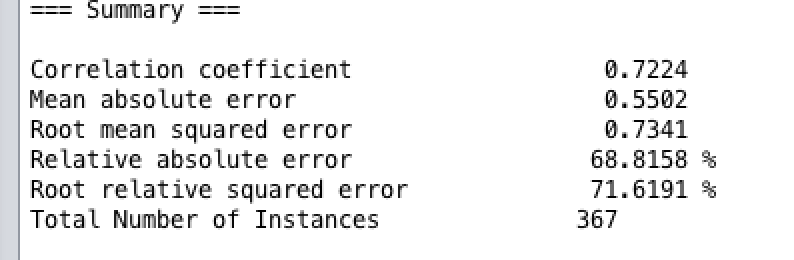
\includegraphics[height=5cm]{imagens/sem_usa_split.png}
\caption{Sem filmes dos EUA e usando \textit{percentage split}}
\label{nousasplit}
\end{figure}


Em seguida, a outra hipótese levantada é de que o investimento feito no filme tem influência na nota final. A figura \ref{nobudgetcv} mostra um erro de 0.7496, utilizando \textit{cross-validation} e a figura \ref{nobudgetsplit} mostra um erro de 0.7235. Mesmo o erro sendo um pouco menor, a diferença no erro entre os resultados obtidos nessa avaliação e com todos os dados, também é pequena demais para poder ser de alguma significância.

\begin{figure}[H]
\centering
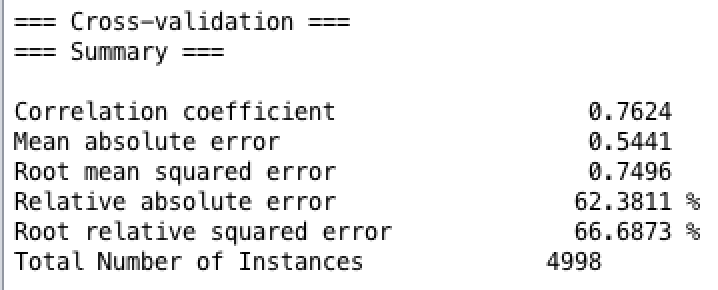
\includegraphics[height=5cm]{imagens/no_budget_cv.png}
\caption{Sem a coluna de orçamento e usando \textit{cross-validation}}
\label{nobudgetcv}
\end{figure}

\begin{figure}[H]
\centering
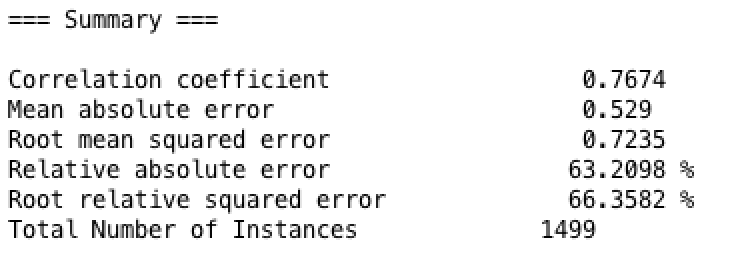
\includegraphics[height=5cm]{imagens/no_budget_split.png}
\caption{Sem a coluna de orçamento e usando \textit{percentage split}}
\label{nobudgetsplit}
\end{figure}


Uma outra hipótese é que o país vai ter influência nos resultados das notas dos filmes. Para testar essa afirmação, a coluna de países foi removida e o mesmo algoritmo citado anteriormente foi usado. A figura \ref{nocountrycv} mostra um RMSE de 0.7462, com \textit{cross validation}. Já a figura \ref{nocountrysplit}, que é com o método \textit{percentage split}, mostra um RMSE de 0.7313. Comparando com os resultados do \textit{dataset} inteiro, é possível concluir que o país tem sim certa influência na nota, mas é muito pouca para ser significativa. 

\begin{figure}[H]
\centering
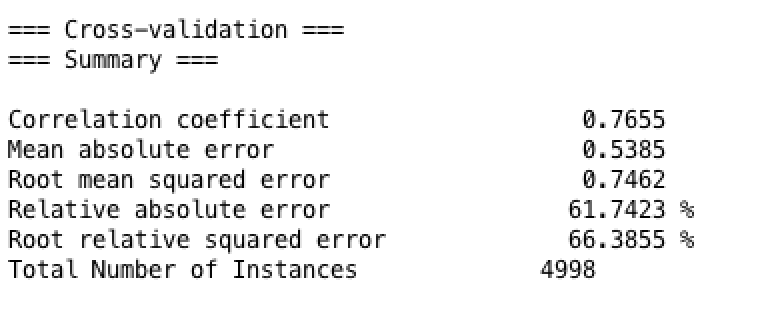
\includegraphics[height=5cm]{imagens/no_country_cv.png}
\caption{Sem a coluna de país e usando \textit{cross-validation}}
\label{nocountrycv}
\end{figure}

\begin{figure}[H]
\centering
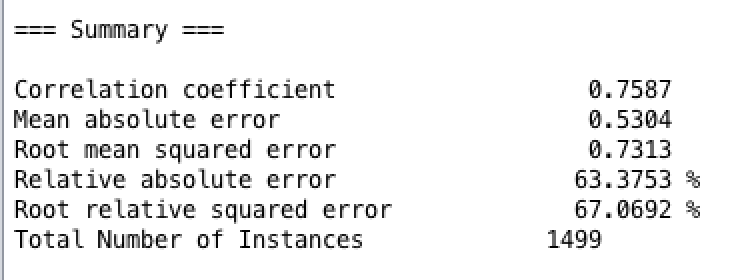
\includegraphics[height=5cm]{imagens/no_country_split.png}
\caption{Sem a coluna de país e usando \textit{percentage split}}
\label{nocountrysplit}
\end{figure}


Por último, a hipótese de que o diretor pode influenciar foi testada. Primeiro, com \textit{cross-validation} como mostra a figura \ref{nodirectorcv} tem um erro de 0.7451, já com \textit{percentage split}, tem um erro de 0.7264, como mostra a figura \ref{nodirectorsplit}. Com o método \textit{cross-validation} o erro foi menor, já usando \textit{percentage split} o erro foi um pouco maior, 0.0019. Isso mostra que o diretor escolhido para dirigir o filme não tem tanta influência na nota do filme. 

\begin{figure}[H]
\centering
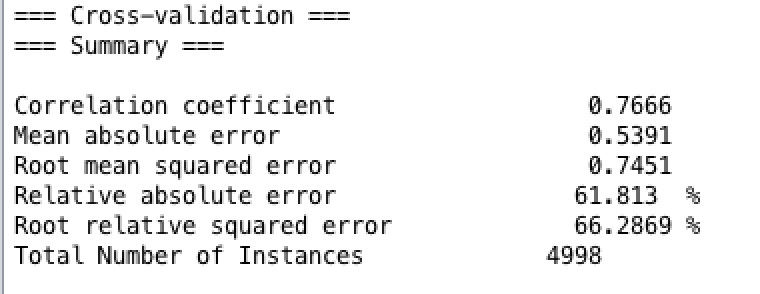
\includegraphics[height=5cm]{imagens/no_director_cv.png}
\caption{Sem a coluna de diretor e usando \textit{cross-validation}}
\label{nodirectorcv}
\end{figure}

\begin{figure}[H]
\centering
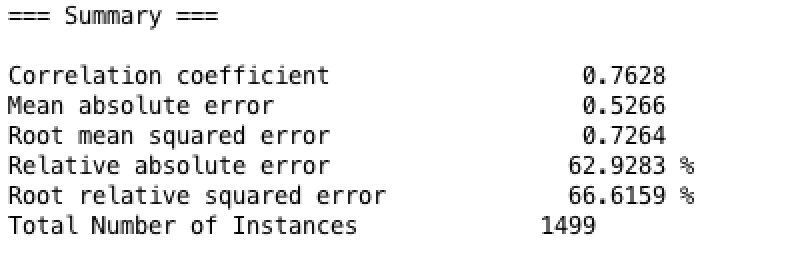
\includegraphics[height=5cm]{imagens/no_director_split.png}
\caption{Sem a coluna de diretor e usando \textit{percentage split}}
\label{nodirectorsplit}
\end{figure}

Dentre todas as hipóteses levantadas, apenas a primeira pôde ser testada com maior precisão, a de prever a nota dos filmes. Utilizando \textit{random forest} e realizando o tratamento dos dados descritos nessa seção, foi possível chegar a um erro de 0.7748, com \textit{cross-validation} (tabela \ref{cvfull}) e 0.7245 usando \textit{percentage split} (tabela \ref{splitfull}). 

\section{CONCLUSÕES}
À luz dos resultados encontrados, é possível concluir que prever as notas de um filme é um trabalho um tanto complicado. Diversas observações e transformações precisam ser realizadas para se ter um resultado apropriado. Além de que uma maior quantidade de amostras seria ideal também.

Diante disso, o trabalho aqui realizado foi capaz de prever as notas com um erro relativamente baixo, de aproximadamente 0.7245, usando \textit{percentage split}. Foi difícil saber com certeza se outros atributos tinham uma influência direta no resultado final, visto que a variação no resultado era muito pouca. Removendo individualmente os atributos de país, diretor e orçamento, o RMSE final variou muito pouco, fazendo com que qualquer conclusão seja imprecisa.

Não foi possível definir se os dados estavam ou não enviesados sem uma observação maior deles, já que o erro, no caso da análise sem os filmes feitos nos Estados Unidos, foi menor. Além de que, sem as produções feitas nos EUA, a quantidade de registros cai de 4998 para 1224, perdendo muitos dados que são de grande importância para a análise de regressão.

Um sistema de recomendações utilizando os resultados desse trabalho é uma possível extensão desse projeto. O sistema poderia levar em consideração a nota que o usuário deu para certos filmes e os gêneros deles, podendo indicar um com uma chance maior de acerto, ou seja, de agradar o usuário.

Além disso, o sistema poderia ajudar a escolher atrizes que têm uma maior influência nas notas, evitando fazer uma escolha possivelmente ruim.
%%%%%%%%%%%%%%%%%%%%%%%%%%%%% Referências 

\nocite{*}
\bibliography{references} 
\bibliographystyle{plain}
%%%%%%%%%%%%%%%%%%%%%%%%%%%%%%%%%%%%%%%%%%%%%%%%%%%%%%%%%%%%%%%%%%%%%%%


\end{document}